\documentclass[twoside]{book}

% Packages required by doxygen
\usepackage{fixltx2e}
\usepackage{calc}
\usepackage{doxygen}
\usepackage[export]{adjustbox} % also loads graphicx
\usepackage{graphicx}
\usepackage[utf8]{inputenc}
\usepackage{makeidx}
\usepackage{multicol}
\usepackage{multirow}
\PassOptionsToPackage{warn}{textcomp}
\usepackage{textcomp}
\usepackage[nointegrals]{wasysym}
\usepackage[table]{xcolor}

% Font selection
\usepackage[T1]{fontenc}
\usepackage[scaled=.90]{helvet}
\usepackage{courier}
\usepackage{amssymb}
\usepackage{sectsty}
\renewcommand{\familydefault}{\sfdefault}
\allsectionsfont{%
  \fontseries{bc}\selectfont%
  \color{darkgray}%
}
\renewcommand{\DoxyLabelFont}{%
  \fontseries{bc}\selectfont%
  \color{darkgray}%
}
\newcommand{\+}{\discretionary{\mbox{\scriptsize$\hookleftarrow$}}{}{}}

% Page & text layout
\usepackage{geometry}
\geometry{%
  a4paper,%
  top=2.5cm,%
  bottom=2.5cm,%
  left=2.5cm,%
  right=2.5cm%
}
\tolerance=750
\hfuzz=15pt
\hbadness=750
\setlength{\emergencystretch}{15pt}
\setlength{\parindent}{0cm}
\setlength{\parskip}{3ex plus 2ex minus 2ex}
\makeatletter
\renewcommand{\paragraph}{%
  \@startsection{paragraph}{4}{0ex}{-1.0ex}{1.0ex}{%
    \normalfont\normalsize\bfseries\SS@parafont%
  }%
}
\renewcommand{\subparagraph}{%
  \@startsection{subparagraph}{5}{0ex}{-1.0ex}{1.0ex}{%
    \normalfont\normalsize\bfseries\SS@subparafont%
  }%
}
\makeatother

% Headers & footers
\usepackage{fancyhdr}
\pagestyle{fancyplain}
\fancyhead[LE]{\fancyplain{}{\bfseries\thepage}}
\fancyhead[CE]{\fancyplain{}{}}
\fancyhead[RE]{\fancyplain{}{\bfseries\leftmark}}
\fancyhead[LO]{\fancyplain{}{\bfseries\rightmark}}
\fancyhead[CO]{\fancyplain{}{}}
\fancyhead[RO]{\fancyplain{}{\bfseries\thepage}}
\fancyfoot[LE]{\fancyplain{}{}}
\fancyfoot[CE]{\fancyplain{}{}}
\fancyfoot[RE]{\fancyplain{}{\bfseries\scriptsize Generated by Doxygen }}
\fancyfoot[LO]{\fancyplain{}{\bfseries\scriptsize Generated by Doxygen }}
\fancyfoot[CO]{\fancyplain{}{}}
\fancyfoot[RO]{\fancyplain{}{}}
\renewcommand{\footrulewidth}{0.4pt}
\renewcommand{\chaptermark}[1]{%
  \markboth{#1}{}%
}
\renewcommand{\sectionmark}[1]{%
  \markright{\thesection\ #1}%
}

% Indices & bibliography
\usepackage{natbib}
\usepackage[titles]{tocloft}
\setcounter{tocdepth}{3}
\setcounter{secnumdepth}{5}
\makeindex

% Hyperlinks (required, but should be loaded last)
\usepackage{ifpdf}
\ifpdf
  \usepackage[pdftex,pagebackref=true]{hyperref}
\else
  \usepackage[ps2pdf,pagebackref=true]{hyperref}
\fi
\hypersetup{%
  colorlinks=true,%
  linkcolor=blue,%
  citecolor=blue,%
  unicode%
}

% Custom commands
\newcommand{\clearemptydoublepage}{%
  \newpage{\pagestyle{empty}\cleardoublepage}%
}

\usepackage{caption}
\captionsetup{labelsep=space,justification=centering,font={bf},singlelinecheck=off,skip=4pt,position=top}

%===== C O N T E N T S =====

\begin{document}

% Titlepage & ToC
\hypersetup{pageanchor=false,
             bookmarksnumbered=true,
             pdfencoding=unicode
            }
\pagenumbering{alph}
\begin{titlepage}
\vspace*{7cm}
\begin{center}%
{\Large Pillar3D }\\
\vspace*{1cm}
{\large Generated by Doxygen 1.8.13}\\
\end{center}
\end{titlepage}
\clearemptydoublepage
\pagenumbering{roman}
\tableofcontents
\clearemptydoublepage
\pagenumbering{arabic}
\hypersetup{pageanchor=true}

%--- Begin generated contents ---
\chapter{Namespace Index}
\section{Packages}
Here are the packages with brief descriptions (if available)\+:\begin{DoxyCompactList}
\item\contentsline{section}{\hyperlink{namespace_pillar3_d}{Pillar3D} }{\pageref{namespace_pillar3_d}}{}
\item\contentsline{section}{\hyperlink{namespace_pillar3_d_1_1_coroutines}{Pillar3\+D.\+Coroutines} }{\pageref{namespace_pillar3_d_1_1_coroutines}}{}
\item\contentsline{section}{\hyperlink{namespace_pillar3_d_1_1_internal}{Pillar3\+D.\+Internal} }{\pageref{namespace_pillar3_d_1_1_internal}}{}
\item\contentsline{section}{\hyperlink{namespace_pillar3_d_1_1_rendering}{Pillar3\+D.\+Rendering} }{\pageref{namespace_pillar3_d_1_1_rendering}}{}
\end{DoxyCompactList}

\chapter{Hierarchical Index}
\section{Class Hierarchy}
This inheritance list is sorted roughly, but not completely, alphabetically\+:\begin{DoxyCompactList}
\item \contentsline{section}{Pillar3\+D.\+Application}{\pageref{class_pillar3_d_1_1_application}}{}
\item \contentsline{section}{Pillar3\+D.\+Component}{\pageref{class_pillar3_d_1_1_component}}{}
\begin{DoxyCompactList}
\item \contentsline{section}{Pillar3\+D.\+Pillar\+Behaviour}{\pageref{class_pillar3_d_1_1_pillar_behaviour}}{}
\item \contentsline{section}{Pillar3\+D.\+Transform}{\pageref{class_pillar3_d_1_1_transform}}{}
\item \contentsline{section}{Sample\+Component}{\pageref{class_sample_component}}{}
\end{DoxyCompactList}
\item \contentsline{section}{Pillar3\+D.\+Entity}{\pageref{class_pillar3_d_1_1_entity}}{}
\item \contentsline{section}{Pillar3\+D.\+Input.\+Input\+Axis}{\pageref{class_pillar3_d_1_1_input_1_1_input_axis}}{}
\item \contentsline{section}{Pillar3\+D.\+Input.\+Input\+Vector2D}{\pageref{class_pillar3_d_1_1_input_1_1_input_vector2_d}}{}
\begin{DoxyCompactList}
\item \contentsline{section}{Pillar3\+D.\+Input.\+Input\+Vector3D}{\pageref{class_pillar3_d_1_1_input_1_1_input_vector3_d}}{}
\end{DoxyCompactList}
\item \contentsline{section}{Pillar3\+D.\+Level}{\pageref{class_pillar3_d_1_1_level}}{}
\item \contentsline{section}{Pillar3\+D.\+Matrix}{\pageref{class_pillar3_d_1_1_matrix}}{}
\begin{DoxyCompactList}
\item \contentsline{section}{Pillar3\+D.\+Matrix4x4}{\pageref{class_pillar3_d_1_1_matrix4x4}}{}
\end{DoxyCompactList}
\item \contentsline{section}{Pillar3\+D.\+Quaternion}{\pageref{class_pillar3_d_1_1_quaternion}}{}
\item \contentsline{section}{Pillar3\+D.\+Rails}{\pageref{class_pillar3_d_1_1_rails}}{}
\item \contentsline{section}{Pillar3\+D.\+Routine\+Runner}{\pageref{class_pillar3_d_1_1_routine_runner}}{}
\item \contentsline{section}{Pillar3\+D.\+Settings}{\pageref{class_pillar3_d_1_1_settings}}{}
\item \contentsline{section}{Pillar3\+D.\+Smart\+Cache$<$ T $>$}{\pageref{class_pillar3_d_1_1_smart_cache}}{}
\item \contentsline{section}{Pillar3\+D.\+Smart\+Cache$<$ Pillar3\+D.\+Quaternion $>$}{\pageref{class_pillar3_d_1_1_smart_cache}}{}
\item \contentsline{section}{Pillar3\+D.\+Smart\+Cache$<$ Pillar3\+D.\+Vector3 $>$}{\pageref{class_pillar3_d_1_1_smart_cache}}{}
\item \contentsline{section}{Test\+Class}{\pageref{class_test_class}}{}
\item \contentsline{section}{Pillar3\+D.\+Thread\+Manager}{\pageref{class_pillar3_d_1_1_thread_manager}}{}
\item \contentsline{section}{Pillar3\+D.\+Time}{\pageref{class_pillar3_d_1_1_time}}{}
\item \contentsline{section}{Pillar3\+D.\+Internal.\+Tracked\+Thread}{\pageref{class_pillar3_d_1_1_internal_1_1_tracked_thread}}{}
\item \contentsline{section}{Pillar3\+D.\+Vector2}{\pageref{class_pillar3_d_1_1_vector2}}{}
\begin{DoxyCompactList}
\item \contentsline{section}{Pillar3\+D.\+Vector3}{\pageref{class_pillar3_d_1_1_vector3}}{}
\begin{DoxyCompactList}
\item \contentsline{section}{Pillar3\+D.\+Vector4}{\pageref{class_pillar3_d_1_1_vector4}}{}
\end{DoxyCompactList}
\end{DoxyCompactList}
\item \contentsline{section}{Pillar3\+D.\+VectorN}{\pageref{class_pillar3_d_1_1_vector_n}}{}
\item \contentsline{section}{Pillar3\+D.\+Rendering.\+Vulkan\+Wrapper}{\pageref{class_pillar3_d_1_1_rendering_1_1_vulkan_wrapper}}{}
\item \contentsline{section}{Pillar3\+D.\+Yield\+Instruction}{\pageref{class_pillar3_d_1_1_yield_instruction}}{}
\begin{DoxyCompactList}
\item \contentsline{section}{Pillar3\+D.\+Coroutines.\+Wait\+For\+Seconds}{\pageref{class_pillar3_d_1_1_coroutines_1_1_wait_for_seconds}}{}
\item \contentsline{section}{Pillar3\+D.\+Coroutines.\+Wait\+For\+Seconds\+Accurate}{\pageref{class_pillar3_d_1_1_coroutines_1_1_wait_for_seconds_accurate}}{}
\item \contentsline{section}{Pillar3\+D.\+Coroutines.\+Wait\+For\+Seconds\+Functional}{\pageref{class_pillar3_d_1_1_coroutines_1_1_wait_for_seconds_functional}}{}
\item \contentsline{section}{Pillar3\+D.\+Coroutines.\+Wait\+For\+Seconds\+Interruptable}{\pageref{class_pillar3_d_1_1_coroutines_1_1_wait_for_seconds_interruptable}}{}
\item \contentsline{section}{Pillar3\+D.\+Coroutines.\+Wait\+For\+Seconds\+Unscaled}{\pageref{class_pillar3_d_1_1_coroutines_1_1_wait_for_seconds_unscaled}}{}
\item \contentsline{section}{Pillar3\+D.\+Coroutines.\+Wait\+Until}{\pageref{class_pillar3_d_1_1_coroutines_1_1_wait_until}}{}
\item \contentsline{section}{Pillar3\+D.\+Coroutines.\+Wait\+While}{\pageref{class_pillar3_d_1_1_coroutines_1_1_wait_while}}{}
\end{DoxyCompactList}
\end{DoxyCompactList}

\chapter{Class Index}
\section{Class List}
Here are the classes, structs, unions and interfaces with brief descriptions\+:\begin{DoxyCompactList}
\item\contentsline{section}{\hyperlink{class_pillar3_d_1_1_application}{Pillar3\+D.\+Application} }{\pageref{class_pillar3_d_1_1_application}}{}
\item\contentsline{section}{\hyperlink{class_pillar3_d_1_1_component}{Pillar3\+D.\+Component} }{\pageref{class_pillar3_d_1_1_component}}{}
\item\contentsline{section}{\hyperlink{class_pillar3_d_1_1_entity}{Pillar3\+D.\+Entity} }{\pageref{class_pillar3_d_1_1_entity}}{}
\item\contentsline{section}{\hyperlink{class_pillar3_d_1_1_input_1_1_input_axis}{Pillar3\+D.\+Input.\+Input\+Axis} }{\pageref{class_pillar3_d_1_1_input_1_1_input_axis}}{}
\item\contentsline{section}{\hyperlink{class_pillar3_d_1_1_input_1_1_input_vector2_d}{Pillar3\+D.\+Input.\+Input\+Vector2D} }{\pageref{class_pillar3_d_1_1_input_1_1_input_vector2_d}}{}
\item\contentsline{section}{\hyperlink{class_pillar3_d_1_1_input_1_1_input_vector3_d}{Pillar3\+D.\+Input.\+Input\+Vector3D} }{\pageref{class_pillar3_d_1_1_input_1_1_input_vector3_d}}{}
\item\contentsline{section}{\hyperlink{class_pillar3_d_1_1_level}{Pillar3\+D.\+Level} }{\pageref{class_pillar3_d_1_1_level}}{}
\item\contentsline{section}{\hyperlink{class_pillar3_d_1_1_matrix}{Pillar3\+D.\+Matrix} }{\pageref{class_pillar3_d_1_1_matrix}}{}
\item\contentsline{section}{\hyperlink{class_pillar3_d_1_1_matrix4x4}{Pillar3\+D.\+Matrix4x4} }{\pageref{class_pillar3_d_1_1_matrix4x4}}{}
\item\contentsline{section}{\hyperlink{class_pillar3_d_1_1_pillar_behaviour}{Pillar3\+D.\+Pillar\+Behaviour} }{\pageref{class_pillar3_d_1_1_pillar_behaviour}}{}
\item\contentsline{section}{\hyperlink{class_pillar3_d_1_1_quaternion}{Pillar3\+D.\+Quaternion} }{\pageref{class_pillar3_d_1_1_quaternion}}{}
\item\contentsline{section}{\hyperlink{class_pillar3_d_1_1_rails}{Pillar3\+D.\+Rails} }{\pageref{class_pillar3_d_1_1_rails}}{}
\item\contentsline{section}{\hyperlink{class_pillar3_d_1_1_routine_runner}{Pillar3\+D.\+Routine\+Runner} }{\pageref{class_pillar3_d_1_1_routine_runner}}{}
\item\contentsline{section}{\hyperlink{class_sample_component}{Sample\+Component} }{\pageref{class_sample_component}}{}
\item\contentsline{section}{\hyperlink{class_pillar3_d_1_1_settings}{Pillar3\+D.\+Settings} }{\pageref{class_pillar3_d_1_1_settings}}{}
\item\contentsline{section}{\hyperlink{class_pillar3_d_1_1_smart_cache}{Pillar3\+D.\+Smart\+Cache$<$ T $>$} }{\pageref{class_pillar3_d_1_1_smart_cache}}{}
\item\contentsline{section}{\hyperlink{class_test_class}{Test\+Class} }{\pageref{class_test_class}}{}
\item\contentsline{section}{\hyperlink{class_pillar3_d_1_1_thread_manager}{Pillar3\+D.\+Thread\+Manager} }{\pageref{class_pillar3_d_1_1_thread_manager}}{}
\item\contentsline{section}{\hyperlink{class_pillar3_d_1_1_time}{Pillar3\+D.\+Time} }{\pageref{class_pillar3_d_1_1_time}}{}
\item\contentsline{section}{\hyperlink{class_pillar3_d_1_1_internal_1_1_tracked_thread}{Pillar3\+D.\+Internal.\+Tracked\+Thread} }{\pageref{class_pillar3_d_1_1_internal_1_1_tracked_thread}}{}
\item\contentsline{section}{\hyperlink{class_pillar3_d_1_1_transform}{Pillar3\+D.\+Transform} }{\pageref{class_pillar3_d_1_1_transform}}{}
\item\contentsline{section}{\hyperlink{class_pillar3_d_1_1_vector2}{Pillar3\+D.\+Vector2} }{\pageref{class_pillar3_d_1_1_vector2}}{}
\item\contentsline{section}{\hyperlink{class_pillar3_d_1_1_vector3}{Pillar3\+D.\+Vector3} }{\pageref{class_pillar3_d_1_1_vector3}}{}
\item\contentsline{section}{\hyperlink{class_pillar3_d_1_1_vector4}{Pillar3\+D.\+Vector4} }{\pageref{class_pillar3_d_1_1_vector4}}{}
\item\contentsline{section}{\hyperlink{class_pillar3_d_1_1_vector_n}{Pillar3\+D.\+VectorN} }{\pageref{class_pillar3_d_1_1_vector_n}}{}
\item\contentsline{section}{\hyperlink{class_pillar3_d_1_1_rendering_1_1_vulkan_wrapper}{Pillar3\+D.\+Rendering.\+Vulkan\+Wrapper} }{\pageref{class_pillar3_d_1_1_rendering_1_1_vulkan_wrapper}}{}
\item\contentsline{section}{\hyperlink{class_pillar3_d_1_1_coroutines_1_1_wait_for_seconds}{Pillar3\+D.\+Coroutines.\+Wait\+For\+Seconds} }{\pageref{class_pillar3_d_1_1_coroutines_1_1_wait_for_seconds}}{}
\item\contentsline{section}{\hyperlink{class_pillar3_d_1_1_coroutines_1_1_wait_for_seconds_accurate}{Pillar3\+D.\+Coroutines.\+Wait\+For\+Seconds\+Accurate} }{\pageref{class_pillar3_d_1_1_coroutines_1_1_wait_for_seconds_accurate}}{}
\item\contentsline{section}{\hyperlink{class_pillar3_d_1_1_coroutines_1_1_wait_for_seconds_functional}{Pillar3\+D.\+Coroutines.\+Wait\+For\+Seconds\+Functional} }{\pageref{class_pillar3_d_1_1_coroutines_1_1_wait_for_seconds_functional}}{}
\item\contentsline{section}{\hyperlink{class_pillar3_d_1_1_coroutines_1_1_wait_for_seconds_interruptable}{Pillar3\+D.\+Coroutines.\+Wait\+For\+Seconds\+Interruptable} }{\pageref{class_pillar3_d_1_1_coroutines_1_1_wait_for_seconds_interruptable}}{}
\item\contentsline{section}{\hyperlink{class_pillar3_d_1_1_coroutines_1_1_wait_for_seconds_unscaled}{Pillar3\+D.\+Coroutines.\+Wait\+For\+Seconds\+Unscaled} }{\pageref{class_pillar3_d_1_1_coroutines_1_1_wait_for_seconds_unscaled}}{}
\item\contentsline{section}{\hyperlink{class_pillar3_d_1_1_coroutines_1_1_wait_until}{Pillar3\+D.\+Coroutines.\+Wait\+Until} }{\pageref{class_pillar3_d_1_1_coroutines_1_1_wait_until}}{}
\item\contentsline{section}{\hyperlink{class_pillar3_d_1_1_coroutines_1_1_wait_while}{Pillar3\+D.\+Coroutines.\+Wait\+While} }{\pageref{class_pillar3_d_1_1_coroutines_1_1_wait_while}}{}
\item\contentsline{section}{\hyperlink{class_pillar3_d_1_1_yield_instruction}{Pillar3\+D.\+Yield\+Instruction} }{\pageref{class_pillar3_d_1_1_yield_instruction}}{}
\end{DoxyCompactList}

\chapter{Namespace Documentation}
\hypertarget{namespace_pillar3_d}{}\section{Pillar3D Namespace Reference}
\label{namespace_pillar3_d}\index{Pillar3D@{Pillar3D}}
\subsection*{Namespaces}
\begin{DoxyCompactItemize}
\end{DoxyCompactItemize}
\subsection*{Classes}
\begin{DoxyCompactItemize}
\item 
class \hyperlink{class_pillar3_d_1_1_application}{Application}
\item 
class \hyperlink{class_pillar3_d_1_1_component}{Component}
\item 
class \hyperlink{class_pillar3_d_1_1_entity}{Entity}
\item 
class {\bfseries Input}
\item 
class \hyperlink{class_pillar3_d_1_1_level}{Level}
\item 
class {\bfseries Mathf}
\item 
class \hyperlink{class_pillar3_d_1_1_matrix}{Matrix}
\item 
class \hyperlink{class_pillar3_d_1_1_matrix4x4}{Matrix4x4}
\item 
class \hyperlink{class_pillar3_d_1_1_pillar_behaviour}{Pillar\+Behaviour}
\item 
class \hyperlink{class_pillar3_d_1_1_quaternion}{Quaternion}
\item 
class \hyperlink{class_pillar3_d_1_1_rails}{Rails}
\item 
class \hyperlink{class_pillar3_d_1_1_routine_runner}{Routine\+Runner}
\item 
class \hyperlink{class_pillar3_d_1_1_settings}{Settings}
\item 
class \hyperlink{class_pillar3_d_1_1_smart_cache}{Smart\+Cache}
\item 
class \hyperlink{class_pillar3_d_1_1_thread_manager}{Thread\+Manager}
\item 
class \hyperlink{class_pillar3_d_1_1_time}{Time}
\item 
class \hyperlink{class_pillar3_d_1_1_transform}{Transform}
\item 
class {\bfseries Utilities}
\item 
class \hyperlink{class_pillar3_d_1_1_vector2}{Vector2}
\item 
class \hyperlink{class_pillar3_d_1_1_vector3}{Vector3}
\item 
class \hyperlink{class_pillar3_d_1_1_vector4}{Vector4}
\item 
class \hyperlink{class_pillar3_d_1_1_vector_n}{VectorN}
\item 
class \hyperlink{class_pillar3_d_1_1_yield_instruction}{Yield\+Instruction}
\end{DoxyCompactItemize}
\subsection*{Enumerations}
\begin{DoxyCompactItemize}
\item 
\mbox{\Hypertarget{namespace_pillar3_d_a4a4ed1dde606b890812ff619626301ad}\label{namespace_pillar3_d_a4a4ed1dde606b890812ff619626301ad}} 
enum {\bfseries Sync\+State} \{ {\bfseries Off}, 
{\bfseries Sync\+Threads}, 
{\bfseries Screen\+Refresh}
 \}
\item 
\mbox{\Hypertarget{namespace_pillar3_d_a5d1a35652f19fae4486e397a9a22e146}\label{namespace_pillar3_d_a5d1a35652f19fae4486e397a9a22e146}} 
enum {\bfseries Instruction} \{ {\bfseries wait}, 
{\bfseries resume}, 
{\bfseries exit}
 \}
\end{DoxyCompactItemize}

\hypertarget{namespace_pillar3_d_1_1_coroutines}{}\section{Pillar3\+D.\+Coroutines Namespace Reference}
\label{namespace_pillar3_d_1_1_coroutines}\index{Pillar3\+D.\+Coroutines@{Pillar3\+D.\+Coroutines}}
\subsection*{Classes}
\begin{DoxyCompactItemize}
\item 
class \hyperlink{class_pillar3_d_1_1_coroutines_1_1_wait_for_seconds}{Wait\+For\+Seconds}
\item 
class \hyperlink{class_pillar3_d_1_1_coroutines_1_1_wait_for_seconds_accurate}{Wait\+For\+Seconds\+Accurate}
\item 
class \hyperlink{class_pillar3_d_1_1_coroutines_1_1_wait_for_seconds_functional}{Wait\+For\+Seconds\+Functional}
\item 
class \hyperlink{class_pillar3_d_1_1_coroutines_1_1_wait_for_seconds_interruptable}{Wait\+For\+Seconds\+Interruptable}
\item 
class \hyperlink{class_pillar3_d_1_1_coroutines_1_1_wait_for_seconds_unscaled}{Wait\+For\+Seconds\+Unscaled}
\item 
class \hyperlink{class_pillar3_d_1_1_coroutines_1_1_wait_until}{Wait\+Until}
\item 
class \hyperlink{class_pillar3_d_1_1_coroutines_1_1_wait_while}{Wait\+While}
\end{DoxyCompactItemize}

\hypertarget{namespace_pillar3_d_1_1_internal}{}\section{Pillar3\+D.\+Internal Namespace Reference}
\label{namespace_pillar3_d_1_1_internal}\index{Pillar3\+D.\+Internal@{Pillar3\+D.\+Internal}}
\subsection*{Classes}
\begin{DoxyCompactItemize}
\item 
class \hyperlink{class_pillar3_d_1_1_internal_1_1_tracked_thread}{Tracked\+Thread}
\end{DoxyCompactItemize}

\hypertarget{namespace_pillar3_d_1_1_rendering}{}\section{Pillar3\+D.\+Rendering Namespace Reference}
\label{namespace_pillar3_d_1_1_rendering}\index{Pillar3\+D.\+Rendering@{Pillar3\+D.\+Rendering}}
\subsection*{Classes}
\begin{DoxyCompactItemize}
\item 
class \hyperlink{class_pillar3_d_1_1_rendering_1_1_vulkan_wrapper}{Vulkan\+Wrapper}
\end{DoxyCompactItemize}

\chapter{Class Documentation}
\hypertarget{class_pillar3_d_1_1_application}{}\section{Pillar3\+D.\+Application Class Reference}
\label{class_pillar3_d_1_1_application}\index{Pillar3\+D.\+Application@{Pillar3\+D.\+Application}}
\subsection*{Public Member Functions}
\begin{DoxyCompactItemize}
\item 
\mbox{\Hypertarget{class_pillar3_d_1_1_application_a31248a85b0b3b187f39728706f3ed1c9}\label{class_pillar3_d_1_1_application_a31248a85b0b3b187f39728706f3ed1c9}} 
{\bfseries Application} (string name)
\end{DoxyCompactItemize}
\subsection*{Static Public Attributes}
\begin{DoxyCompactItemize}
\item 
\mbox{\Hypertarget{class_pillar3_d_1_1_application_aaa49c719bd3f8d74f8b1a1bb7a1cf6f9}\label{class_pillar3_d_1_1_application_aaa49c719bd3f8d74f8b1a1bb7a1cf6f9}} 
static int {\bfseries Refresh\+Rate} = 60
\end{DoxyCompactItemize}
\subsection*{Properties}
\begin{DoxyCompactItemize}
\item 
\mbox{\Hypertarget{class_pillar3_d_1_1_application_af6c4035d90799be965e411ec1207c9af}\label{class_pillar3_d_1_1_application_af6c4035d90799be965e411ec1207c9af}} 
static string {\bfseries Version}\hspace{0.3cm}{\ttfamily  \mbox{[}get\mbox{]}}
\item 
\mbox{\Hypertarget{class_pillar3_d_1_1_application_a5effc5fbea9c01a7ed564f9b70e527c6}\label{class_pillar3_d_1_1_application_a5effc5fbea9c01a7ed564f9b70e527c6}} 
static string {\bfseries OS} = \$\char`\"{}Version 0.\+1.\+5\char`\"{}\hspace{0.3cm}{\ttfamily  \mbox{[}get\mbox{]}}
\item 
\mbox{\Hypertarget{class_pillar3_d_1_1_application_ad1c6f009d2706b07f1582145441dd223}\label{class_pillar3_d_1_1_application_ad1c6f009d2706b07f1582145441dd223}} 
static string {\bfseries Name} = Environment.\+O\+S\+Version.\+Platform.\+To\+String()\hspace{0.3cm}{\ttfamily  \mbox{[}get\mbox{]}}
\end{DoxyCompactItemize}


The documentation for this class was generated from the following file\+:\begin{DoxyCompactItemize}
\item 
C\+:/\+Users/gaben/\+Documents/\+Visual Studio 2015/\+Projects/\+Pillar/\+Pillar/\+Internal/Application.\+cs\end{DoxyCompactItemize}

\hypertarget{class_pillar3_d_1_1_component}{}\section{Pillar3\+D.\+Component Class Reference}
\label{class_pillar3_d_1_1_component}\index{Pillar3\+D.\+Component@{Pillar3\+D.\+Component}}
Inheritance diagram for Pillar3\+D.\+Component\+:\begin{figure}[H]
\begin{center}
\leavevmode
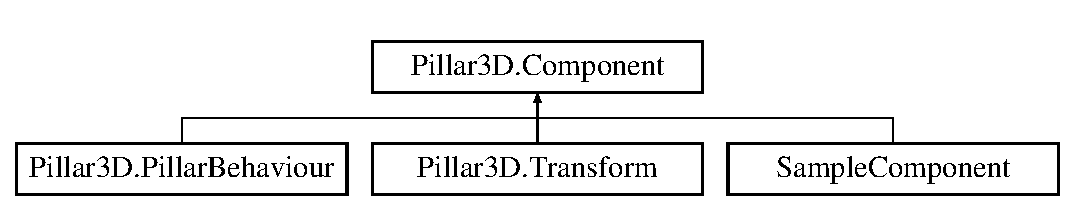
\includegraphics[height=2.000000cm]{class_pillar3_d_1_1_component}
\end{center}
\end{figure}
\subsection*{Public Member Functions}
\begin{DoxyCompactItemize}
\item 
\mbox{\Hypertarget{class_pillar3_d_1_1_component_a7e21ae60e959d9701de58ccf74bcc3b8}\label{class_pillar3_d_1_1_component_a7e21ae60e959d9701de58ccf74bcc3b8}} 
{\bfseries Component} (bool allow\+Multiple)
\item 
\mbox{\Hypertarget{class_pillar3_d_1_1_component_ad275df027f1fd65d5d0a62ee82767985}\label{class_pillar3_d_1_1_component_ad275df027f1fd65d5d0a62ee82767985}} 
virtual void {\bfseries On\+Component\+Added} ()
\item 
\mbox{\Hypertarget{class_pillar3_d_1_1_component_a4efd313fb7d9b3c757a97152cb2b1f4d}\label{class_pillar3_d_1_1_component_a4efd313fb7d9b3c757a97152cb2b1f4d}} 
virtual void {\bfseries On\+Component\+Removed} ()
\end{DoxyCompactItemize}
\subsection*{Static Public Member Functions}
\begin{DoxyCompactItemize}
\item 
\mbox{\Hypertarget{class_pillar3_d_1_1_component_a5c2a2ae3aeb34d2ed0e07651d4829692}\label{class_pillar3_d_1_1_component_a5c2a2ae3aeb34d2ed0e07651d4829692}} 
static \hyperlink{class_pillar3_d_1_1_entity}{Entity} {\bfseries Instantiate} (\hyperlink{class_pillar3_d_1_1_entity}{Entity} original)
\end{DoxyCompactItemize}
\subsection*{Static Public Attributes}
\begin{DoxyCompactItemize}
\item 
\mbox{\Hypertarget{class_pillar3_d_1_1_component_a292ec0044cd5c993b98693fa88682084}\label{class_pillar3_d_1_1_component_a292ec0044cd5c993b98693fa88682084}} 
static bool {\bfseries Allow\+Multiple}
\end{DoxyCompactItemize}
\subsection*{Properties}
\begin{DoxyCompactItemize}
\item 
\mbox{\Hypertarget{class_pillar3_d_1_1_component_af1c87766c5b845e05b496ec7823184a6}\label{class_pillar3_d_1_1_component_af1c87766c5b845e05b496ec7823184a6}} 
int {\bfseries ID}\hspace{0.3cm}{\ttfamily  \mbox{[}get\mbox{]}}
\item 
\mbox{\Hypertarget{class_pillar3_d_1_1_component_a74bee0cc3feb34def0018ba501e5411c}\label{class_pillar3_d_1_1_component_a74bee0cc3feb34def0018ba501e5411c}} 
Action {\bfseries Update}\hspace{0.3cm}{\ttfamily  \mbox{[}get, set\mbox{]}}
\item 
\mbox{\Hypertarget{class_pillar3_d_1_1_component_aef053db26bd22e840c8bf918bcf8c5f3}\label{class_pillar3_d_1_1_component_aef053db26bd22e840c8bf918bcf8c5f3}} 
Action {\bfseries Persistant\+Update}\hspace{0.3cm}{\ttfamily  \mbox{[}get, set\mbox{]}}
\item 
\mbox{\Hypertarget{class_pillar3_d_1_1_component_a8c79529444e423d4e951148e49bc2f33}\label{class_pillar3_d_1_1_component_a8c79529444e423d4e951148e49bc2f33}} 
bool {\bfseries Paused}\hspace{0.3cm}{\ttfamily  \mbox{[}get, set\mbox{]}}
\end{DoxyCompactItemize}


The documentation for this class was generated from the following file\+:\begin{DoxyCompactItemize}
\item 
C\+:/\+Users/gaben/\+Documents/\+Visual Studio 2015/\+Projects/\+Pillar/\+Pillar/\+Internal/Component.\+cs\end{DoxyCompactItemize}

\hypertarget{class_pillar3_d_1_1_entity}{}\section{Pillar3\+D.\+Entity Class Reference}
\label{class_pillar3_d_1_1_entity}\index{Pillar3\+D.\+Entity@{Pillar3\+D.\+Entity}}
\subsection*{Public Member Functions}
\begin{DoxyCompactItemize}
\item 
\mbox{\Hypertarget{class_pillar3_d_1_1_entity_a528c56df6fdb8bef5970863c3642d26b}\label{class_pillar3_d_1_1_entity_a528c56df6fdb8bef5970863c3642d26b}} 
{\bfseries Entity} (string name)
\item 
\mbox{\Hypertarget{class_pillar3_d_1_1_entity_acf50462d86c34af5e6474442bcec5bcb}\label{class_pillar3_d_1_1_entity_acf50462d86c34af5e6474442bcec5bcb}} 
C {\bfseries Add\+Component$<$ C $>$} ()
\item 
C \hyperlink{class_pillar3_d_1_1_entity_aa074e5244bd8980eebc56863a6d77aaf}{Add\+Component$<$ C $>$} (Xml\+Reader defaults)
\begin{DoxyCompactList}\small\item\em Adds component with default data. \end{DoxyCompactList}\item 
\mbox{\Hypertarget{class_pillar3_d_1_1_entity_ab7bd626b58ae21c122e9978e4c2a1cdb}\label{class_pillar3_d_1_1_entity_ab7bd626b58ae21c122e9978e4c2a1cdb}} 
void {\bfseries Remove\+Component$<$ C $>$} ()
\item 
\mbox{\Hypertarget{class_pillar3_d_1_1_entity_ad290b845ff7fe3713b74b35c90942513}\label{class_pillar3_d_1_1_entity_ad290b845ff7fe3713b74b35c90942513}} 
void {\bfseries Set\+Parent} (\hyperlink{class_pillar3_d_1_1_entity}{Entity} parent)
\item 
\mbox{\Hypertarget{class_pillar3_d_1_1_entity_a0a827698ed7b233cf4fe5e6301054fbc}\label{class_pillar3_d_1_1_entity_a0a827698ed7b233cf4fe5e6301054fbc}} 
\hyperlink{class_pillar3_d_1_1_entity}{Entity} {\bfseries Clone} ()
\end{DoxyCompactItemize}
\subsection*{Static Public Member Functions}
\begin{DoxyCompactItemize}
\item 
\mbox{\Hypertarget{class_pillar3_d_1_1_entity_a1be1caaff8af11892461fb9110dc443d}\label{class_pillar3_d_1_1_entity_a1be1caaff8af11892461fb9110dc443d}} 
static \hyperlink{class_pillar3_d_1_1_entity}{Entity} {\bfseries Find\+Entity\+With\+Tag} (string tag)
\item 
\mbox{\Hypertarget{class_pillar3_d_1_1_entity_af0c227ec11474cac19dc026638690761}\label{class_pillar3_d_1_1_entity_af0c227ec11474cac19dc026638690761}} 
static \hyperlink{class_pillar3_d_1_1_entity}{Entity} \mbox{[}$\,$\mbox{]} {\bfseries Find\+Entities\+With\+Tag} (string tag)
\end{DoxyCompactItemize}
\subsection*{Public Attributes}
\begin{DoxyCompactItemize}
\item 
\mbox{\Hypertarget{class_pillar3_d_1_1_entity_af6b3418342679d925906976cd280dc3f}\label{class_pillar3_d_1_1_entity_af6b3418342679d925906976cd280dc3f}} 
List$<$ \hyperlink{class_pillar3_d_1_1_component}{Component} $>$ {\bfseries Components}
\item 
\mbox{\Hypertarget{class_pillar3_d_1_1_entity_add97af29fc9793dd5bdaa537fa6e02bd}\label{class_pillar3_d_1_1_entity_add97af29fc9793dd5bdaa537fa6e02bd}} 
List$<$ \hyperlink{class_pillar3_d_1_1_entity}{Entity} $>$ {\bfseries Children}
\item 
\mbox{\Hypertarget{class_pillar3_d_1_1_entity_a4ca24efa3d85b84349328f04a9d7e906}\label{class_pillar3_d_1_1_entity_a4ca24efa3d85b84349328f04a9d7e906}} 
bool {\bfseries Active}
\item 
\mbox{\Hypertarget{class_pillar3_d_1_1_entity_a1bd147d32ba1424876a66fb742045368}\label{class_pillar3_d_1_1_entity_a1bd147d32ba1424876a66fb742045368}} 
string {\bfseries Name}
\item 
\mbox{\Hypertarget{class_pillar3_d_1_1_entity_a6bd56dd22d22db75aed7bec4afa70f7b}\label{class_pillar3_d_1_1_entity_a6bd56dd22d22db75aed7bec4afa70f7b}} 
Action {\bfseries On\+Parent\+Changed}
\item 
\mbox{\Hypertarget{class_pillar3_d_1_1_entity_a97da2e7efd6600e065d3d6ec6b8d50c0}\label{class_pillar3_d_1_1_entity_a97da2e7efd6600e065d3d6ec6b8d50c0}} 
Action {\bfseries On\+Level\+Changed}
\end{DoxyCompactItemize}
\subsection*{Properties}
\begin{DoxyCompactItemize}
\item 
\mbox{\Hypertarget{class_pillar3_d_1_1_entity_adfc52dc8ac331406e8e4b1532ade729e}\label{class_pillar3_d_1_1_entity_adfc52dc8ac331406e8e4b1532ade729e}} 
\hyperlink{class_pillar3_d_1_1_entity}{Entity} {\bfseries Parent}\hspace{0.3cm}{\ttfamily  \mbox{[}get\mbox{]}}
\item 
\mbox{\Hypertarget{class_pillar3_d_1_1_entity_a3d99069a63a32e59f7504d646f854c2c}\label{class_pillar3_d_1_1_entity_a3d99069a63a32e59f7504d646f854c2c}} 
bool {\bfseries Active\+In\+Tree}\hspace{0.3cm}{\ttfamily  \mbox{[}get\mbox{]}}
\item 
\mbox{\Hypertarget{class_pillar3_d_1_1_entity_a145351b0612b86a83bc2cf7bb8e5b6fa}\label{class_pillar3_d_1_1_entity_a145351b0612b86a83bc2cf7bb8e5b6fa}} 
int {\bfseries ID}\hspace{0.3cm}{\ttfamily  \mbox{[}get\mbox{]}}
\item 
\mbox{\Hypertarget{class_pillar3_d_1_1_entity_adb21c036bafae9305d9d130c12a58ce1}\label{class_pillar3_d_1_1_entity_adb21c036bafae9305d9d130c12a58ce1}} 
\hyperlink{class_pillar3_d_1_1_level}{Level} {\bfseries Container\+Level}\hspace{0.3cm}{\ttfamily  \mbox{[}get\mbox{]}}
\item 
\mbox{\Hypertarget{class_pillar3_d_1_1_entity_aaedc6ef17992adffd4e2f23fc0e8475c}\label{class_pillar3_d_1_1_entity_aaedc6ef17992adffd4e2f23fc0e8475c}} 
string {\bfseries Tag}\hspace{0.3cm}{\ttfamily  \mbox{[}get, set\mbox{]}}
\end{DoxyCompactItemize}


\subsection{Member Function Documentation}
\mbox{\Hypertarget{class_pillar3_d_1_1_entity_aa074e5244bd8980eebc56863a6d77aaf}\label{class_pillar3_d_1_1_entity_aa074e5244bd8980eebc56863a6d77aaf}} 
\index{Pillar3\+D\+::\+Entity@{Pillar3\+D\+::\+Entity}!Add\+Component$<$ C $>$@{Add\+Component$<$ C $>$}}
\index{Add\+Component$<$ C $>$@{Add\+Component$<$ C $>$}!Pillar3\+D\+::\+Entity@{Pillar3\+D\+::\+Entity}}
\subsubsection{\texorpdfstring{Add\+Component$<$ C $>$()}{AddComponent< C >()}}
{\footnotesize\ttfamily C Pillar3\+D.\+Entity.\+Add\+Component$<$ C $>$ (\begin{DoxyParamCaption}\item[{Xml\+Reader}]{defaults }\end{DoxyParamCaption})}



Adds component with default data. 


\begin{DoxyParams}{Parameters}
{\em defaults} & X\+ML data with default data for component\\
\hline
\end{DoxyParams}
\begin{Desc}
\item[Type Constraints]\begin{description}
\item[{\em C} : {\em Component}]\item[{\em C} : {\em new()}]\end{description}
\end{Desc}


The documentation for this class was generated from the following file\+:\begin{DoxyCompactItemize}
\item 
C\+:/\+Users/gaben/\+Documents/\+Visual Studio 2015/\+Projects/\+Pillar/\+Pillar/\+Internal/Entity.\+cs\end{DoxyCompactItemize}

\hypertarget{class_pillar3_d_1_1_input_1_1_input_axis}{}\section{Pillar3\+D.\+Input.\+Input\+Axis Class Reference}
\label{class_pillar3_d_1_1_input_1_1_input_axis}\index{Pillar3\+D.\+Input.\+Input\+Axis@{Pillar3\+D.\+Input.\+Input\+Axis}}
\subsection*{Public Member Functions}
\begin{DoxyCompactItemize}
\item 
\mbox{\Hypertarget{class_pillar3_d_1_1_input_1_1_input_axis_a04ef874c3f288fa704457e80a0e46e39}\label{class_pillar3_d_1_1_input_1_1_input_axis_a04ef874c3f288fa704457e80a0e46e39}} 
{\bfseries Input\+Axis} (Key Negative\+Key, Key Positive\+Key)
\item 
\mbox{\Hypertarget{class_pillar3_d_1_1_input_1_1_input_axis_a800eedc76bf45448b5439e018fd107fc}\label{class_pillar3_d_1_1_input_1_1_input_axis_a800eedc76bf45448b5439e018fd107fc}} 
float {\bfseries Evaluate} ()
\item 
\mbox{\Hypertarget{class_pillar3_d_1_1_input_1_1_input_axis_adb374e448c292493a02915bbd82a0f7e}\label{class_pillar3_d_1_1_input_1_1_input_axis_adb374e448c292493a02915bbd82a0f7e}} 
bool {\bfseries Dead} ()
\end{DoxyCompactItemize}


The documentation for this class was generated from the following file\+:\begin{DoxyCompactItemize}
\item 
C\+:/\+Users/gaben/\+Documents/\+Visual Studio 2015/\+Projects/\+Pillar/\+Pillar/\+Internal/Input.\+cs\end{DoxyCompactItemize}

\hypertarget{class_pillar3_d_1_1_input_1_1_input_vector2_d}{}\section{Pillar3\+D.\+Input.\+Input\+Vector2D Class Reference}
\label{class_pillar3_d_1_1_input_1_1_input_vector2_d}\index{Pillar3\+D.\+Input.\+Input\+Vector2D@{Pillar3\+D.\+Input.\+Input\+Vector2D}}
Inheritance diagram for Pillar3\+D.\+Input.\+Input\+Vector2D\+:\begin{figure}[H]
\begin{center}
\leavevmode
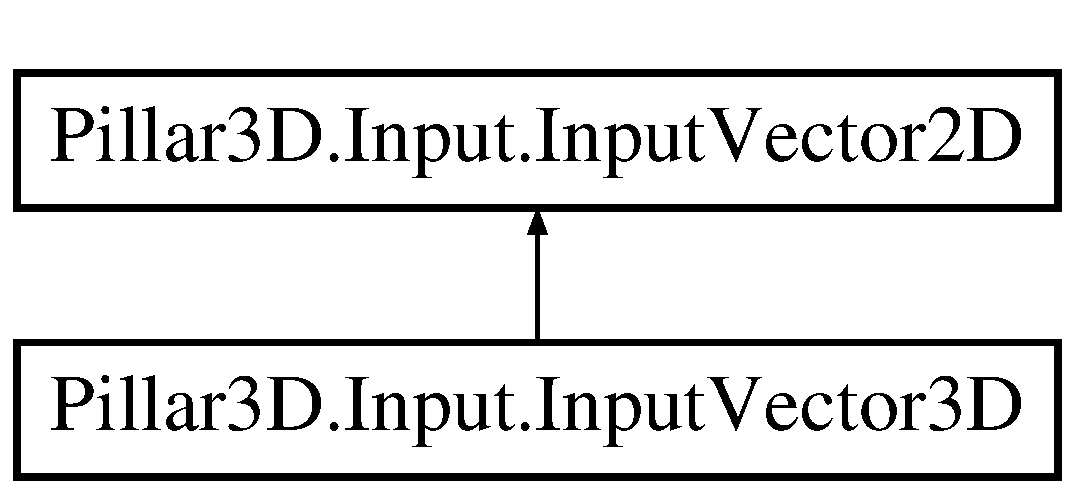
\includegraphics[height=2.000000cm]{class_pillar3_d_1_1_input_1_1_input_vector2_d}
\end{center}
\end{figure}
\subsection*{Public Member Functions}
\begin{DoxyCompactItemize}
\item 
\mbox{\Hypertarget{class_pillar3_d_1_1_input_1_1_input_vector2_d_a8eb3ccb14fd9446243a05d5d62e7f8ba}\label{class_pillar3_d_1_1_input_1_1_input_vector2_d_a8eb3ccb14fd9446243a05d5d62e7f8ba}} 
{\bfseries Input\+Vector2D} (\hyperlink{class_pillar3_d_1_1_input_1_1_input_axis}{Input\+Axis} x, \hyperlink{class_pillar3_d_1_1_input_1_1_input_axis}{Input\+Axis} y)
\item 
\mbox{\Hypertarget{class_pillar3_d_1_1_input_1_1_input_vector2_d_a8da29a7be330061dfe6347d6871887d0}\label{class_pillar3_d_1_1_input_1_1_input_vector2_d_a8da29a7be330061dfe6347d6871887d0}} 
\hyperlink{class_pillar3_d_1_1_vector2}{Vector2} {\bfseries Evaluate} ()
\item 
\mbox{\Hypertarget{class_pillar3_d_1_1_input_1_1_input_vector2_d_a1f9ef3f05ed66987895834c165da2d94}\label{class_pillar3_d_1_1_input_1_1_input_vector2_d_a1f9ef3f05ed66987895834c165da2d94}} 
bool {\bfseries Dead} ()
\end{DoxyCompactItemize}
\subsection*{Public Attributes}
\begin{DoxyCompactItemize}
\item 
\mbox{\Hypertarget{class_pillar3_d_1_1_input_1_1_input_vector2_d_a81509d9a96db00d680d1fb119cb716ab}\label{class_pillar3_d_1_1_input_1_1_input_vector2_d_a81509d9a96db00d680d1fb119cb716ab}} 
\hyperlink{class_pillar3_d_1_1_input_1_1_input_axis}{Input\+Axis} {\bfseries X}
\end{DoxyCompactItemize}


The documentation for this class was generated from the following file\+:\begin{DoxyCompactItemize}
\item 
C\+:/\+Users/gaben/\+Documents/\+Visual Studio 2015/\+Projects/\+Pillar/\+Pillar/\+Internal/Input.\+cs\end{DoxyCompactItemize}

\hypertarget{class_pillar3_d_1_1_input_1_1_input_vector3_d}{}\section{Pillar3\+D.\+Input.\+Input\+Vector3D Class Reference}
\label{class_pillar3_d_1_1_input_1_1_input_vector3_d}\index{Pillar3\+D.\+Input.\+Input\+Vector3D@{Pillar3\+D.\+Input.\+Input\+Vector3D}}
Inheritance diagram for Pillar3\+D.\+Input.\+Input\+Vector3D\+:\begin{figure}[H]
\begin{center}
\leavevmode
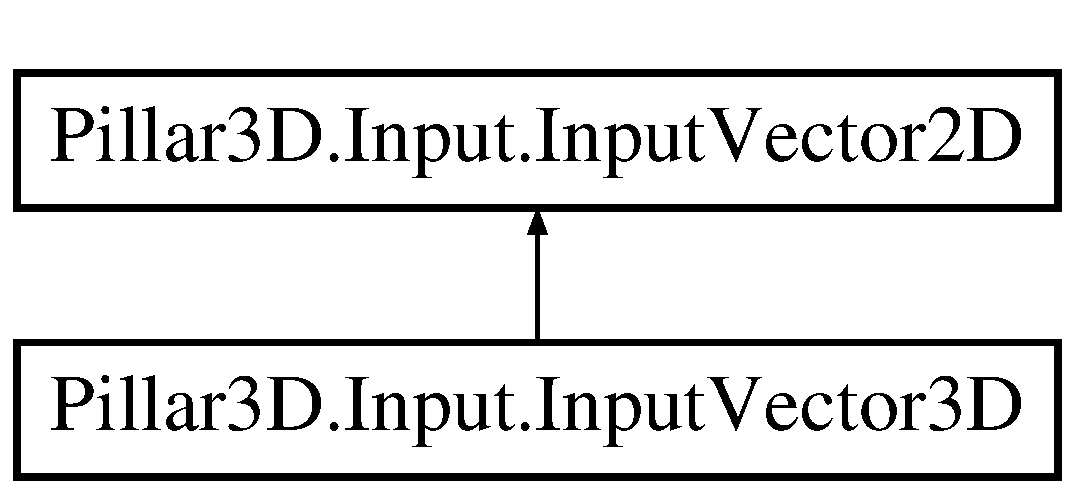
\includegraphics[height=2.000000cm]{class_pillar3_d_1_1_input_1_1_input_vector3_d}
\end{center}
\end{figure}
\subsection*{Public Member Functions}
\begin{DoxyCompactItemize}
\item 
\mbox{\Hypertarget{class_pillar3_d_1_1_input_1_1_input_vector3_d_a72d21323b3e420bd9fdec5b8163827e8}\label{class_pillar3_d_1_1_input_1_1_input_vector3_d_a72d21323b3e420bd9fdec5b8163827e8}} 
{\bfseries Input\+Vector3D} (\hyperlink{class_pillar3_d_1_1_input_1_1_input_axis}{Input\+Axis} x, \hyperlink{class_pillar3_d_1_1_input_1_1_input_axis}{Input\+Axis} y, \hyperlink{class_pillar3_d_1_1_input_1_1_input_axis}{Input\+Axis} z)
\item 
\mbox{\Hypertarget{class_pillar3_d_1_1_input_1_1_input_vector3_d_af4551b218288c9d9cfef295c9668530b}\label{class_pillar3_d_1_1_input_1_1_input_vector3_d_af4551b218288c9d9cfef295c9668530b}} 
new \hyperlink{class_pillar3_d_1_1_vector3}{Vector3} {\bfseries Evaluate} ()
\end{DoxyCompactItemize}
\subsection*{Public Attributes}
\begin{DoxyCompactItemize}
\item 
\mbox{\Hypertarget{class_pillar3_d_1_1_input_1_1_input_vector3_d_a35e4249c283e28d783252b7cc571cba4}\label{class_pillar3_d_1_1_input_1_1_input_vector3_d_a35e4249c283e28d783252b7cc571cba4}} 
\hyperlink{class_pillar3_d_1_1_input_1_1_input_axis}{Input\+Axis} {\bfseries Z}
\end{DoxyCompactItemize}


The documentation for this class was generated from the following file\+:\begin{DoxyCompactItemize}
\item 
C\+:/\+Users/gaben/\+Documents/\+Visual Studio 2015/\+Projects/\+Pillar/\+Pillar/\+Internal/Input.\+cs\end{DoxyCompactItemize}

\hypertarget{class_pillar3_d_1_1_level}{}\section{Pillar3\+D.\+Level Class Reference}
\label{class_pillar3_d_1_1_level}\index{Pillar3\+D.\+Level@{Pillar3\+D.\+Level}}
\subsection*{Public Member Functions}
\begin{DoxyCompactItemize}
\item 
\mbox{\Hypertarget{class_pillar3_d_1_1_level_acdb986304d922d1a7cd2f1c119ce6b8b}\label{class_pillar3_d_1_1_level_acdb986304d922d1a7cd2f1c119ce6b8b}} 
{\bfseries Level} (string name)
\item 
\mbox{\Hypertarget{class_pillar3_d_1_1_level_a0a70a720b583904cb057ced5ac94ed77}\label{class_pillar3_d_1_1_level_a0a70a720b583904cb057ced5ac94ed77}} 
{\bfseries Level} (string name, int thread)
\item 
\mbox{\Hypertarget{class_pillar3_d_1_1_level_a8edca107e635454b6b069c31a795ab30}\label{class_pillar3_d_1_1_level_a8edca107e635454b6b069c31a795ab30}} 
{\bfseries Level} (Xml\+Reader defaults)
\item 
\mbox{\Hypertarget{class_pillar3_d_1_1_level_a1a1cefe13861a4d3412c92c18d03e7f1}\label{class_pillar3_d_1_1_level_a1a1cefe13861a4d3412c92c18d03e7f1}} 
void {\bfseries Frame} ()
\item 
\mbox{\Hypertarget{class_pillar3_d_1_1_level_a66afd3c9ed001bfbe0f416f47665b045}\label{class_pillar3_d_1_1_level_a66afd3c9ed001bfbe0f416f47665b045}} 
int {\bfseries Get\+Stress} ()
\end{DoxyCompactItemize}
\subsection*{Public Attributes}
\begin{DoxyCompactItemize}
\item 
\mbox{\Hypertarget{class_pillar3_d_1_1_level_a931ebe02f1e1efab09139e3be3b860fa}\label{class_pillar3_d_1_1_level_a931ebe02f1e1efab09139e3be3b860fa}} 
\hyperlink{class_pillar3_d_1_1_entity}{Entity} {\bfseries Root}
\item 
\mbox{\Hypertarget{class_pillar3_d_1_1_level_a387ffc78f30fe32077aa04bb379f74f0}\label{class_pillar3_d_1_1_level_a387ffc78f30fe32077aa04bb379f74f0}} 
string {\bfseries Name}
\item 
\mbox{\Hypertarget{class_pillar3_d_1_1_level_a25a420f2a393d22c79a4acf62f278945}\label{class_pillar3_d_1_1_level_a25a420f2a393d22c79a4acf62f278945}} 
\hyperlink{class_pillar3_d_1_1_rails}{Rails} {\bfseries Rail}
\end{DoxyCompactItemize}
\subsection*{Static Public Attributes}
\begin{DoxyCompactItemize}
\item 
\mbox{\Hypertarget{class_pillar3_d_1_1_level_a6ebfe0dcd9467a921473d1d65bd81e79}\label{class_pillar3_d_1_1_level_a6ebfe0dcd9467a921473d1d65bd81e79}} 
static \hyperlink{class_pillar3_d_1_1_level}{Level} {\bfseries Main\+Level}
\end{DoxyCompactItemize}


The documentation for this class was generated from the following file\+:\begin{DoxyCompactItemize}
\item 
C\+:/\+Users/gaben/\+Documents/\+Visual Studio 2015/\+Projects/\+Pillar/\+Pillar/\+Internal/Level.\+cs\end{DoxyCompactItemize}

\hypertarget{class_pillar3_d_1_1_matrix}{}\section{Pillar3\+D.\+Matrix Class Reference}
\label{class_pillar3_d_1_1_matrix}\index{Pillar3\+D.\+Matrix@{Pillar3\+D.\+Matrix}}
Inheritance diagram for Pillar3\+D.\+Matrix\+:\begin{figure}[H]
\begin{center}
\leavevmode
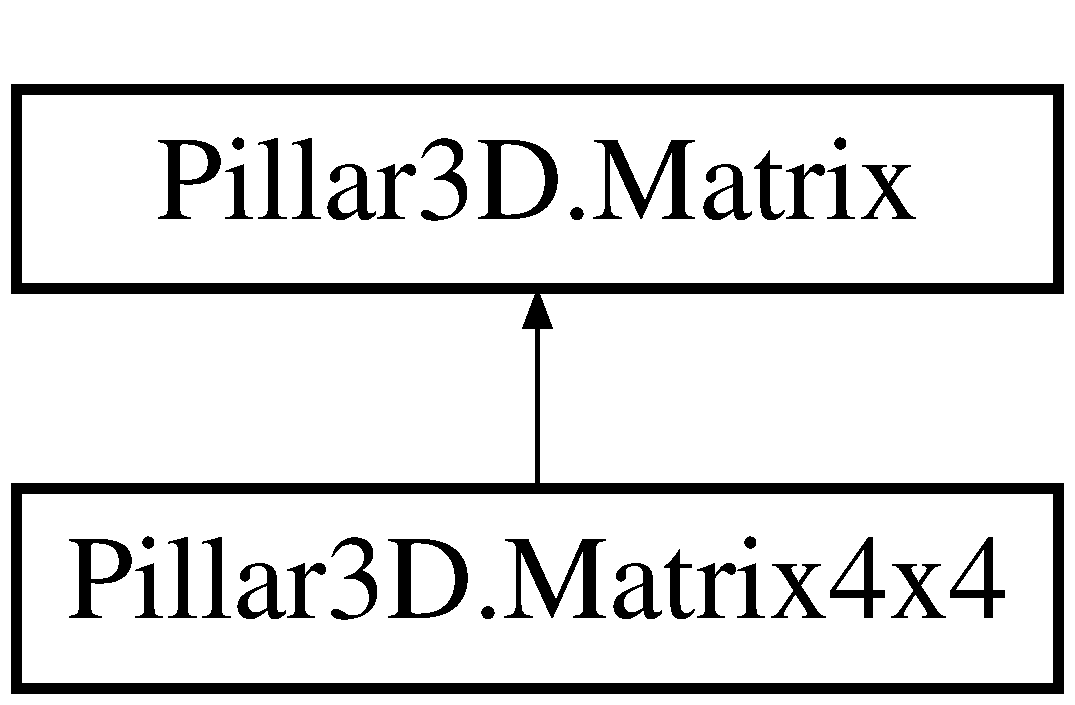
\includegraphics[height=2.000000cm]{class_pillar3_d_1_1_matrix}
\end{center}
\end{figure}
\subsection*{Public Member Functions}
\begin{DoxyCompactItemize}
\item 
\mbox{\Hypertarget{class_pillar3_d_1_1_matrix_a64beebf9fcf02359cef7c67192b9ed2a}\label{class_pillar3_d_1_1_matrix_a64beebf9fcf02359cef7c67192b9ed2a}} 
{\bfseries Matrix} (int rows, int columns)
\item 
\mbox{\Hypertarget{class_pillar3_d_1_1_matrix_ab235003e1b5247725d21d31d78b36d8f}\label{class_pillar3_d_1_1_matrix_ab235003e1b5247725d21d31d78b36d8f}} 
{\bfseries Matrix} (float\mbox{[}$\,$\mbox{]}\mbox{[}$\,$\mbox{]} values)
\item 
\mbox{\Hypertarget{class_pillar3_d_1_1_matrix_aef7d44611db4397544f49ca8033cfee0}\label{class_pillar3_d_1_1_matrix_aef7d44611db4397544f49ca8033cfee0}} 
float {\bfseries Determinant} ()
\item 
\mbox{\Hypertarget{class_pillar3_d_1_1_matrix_a4dfa66ec81485f719f0d27056cd73a46}\label{class_pillar3_d_1_1_matrix_a4dfa66ec81485f719f0d27056cd73a46}} 
float {\bfseries Trace} ()
\item 
\mbox{\Hypertarget{class_pillar3_d_1_1_matrix_a65c68040c1e23a49cf9d9e3372357ec4}\label{class_pillar3_d_1_1_matrix_a65c68040c1e23a49cf9d9e3372357ec4}} 
\hyperlink{class_pillar3_d_1_1_matrix}{Matrix} {\bfseries Transpose} ()
\item 
\mbox{\Hypertarget{class_pillar3_d_1_1_matrix_a7ffcc88bea24885317f5fdb7da79607f}\label{class_pillar3_d_1_1_matrix_a7ffcc88bea24885317f5fdb7da79607f}} 
\hyperlink{class_pillar3_d_1_1_matrix}{Matrix} {\bfseries Get\+Exclusionary\+Matrix} (int row, int column)
\item 
\mbox{\Hypertarget{class_pillar3_d_1_1_matrix_a935dcbdbfb9c78de7edecee966009926}\label{class_pillar3_d_1_1_matrix_a935dcbdbfb9c78de7edecee966009926}} 
\hyperlink{class_pillar3_d_1_1_vector_n}{VectorN} {\bfseries Get\+Column} (int column)
\item 
\mbox{\Hypertarget{class_pillar3_d_1_1_matrix_a8a18678e237023687dd21994d57d144b}\label{class_pillar3_d_1_1_matrix_a8a18678e237023687dd21994d57d144b}} 
\hyperlink{class_pillar3_d_1_1_vector_n}{VectorN} {\bfseries Get\+Row} (int row)
\item 
\mbox{\Hypertarget{class_pillar3_d_1_1_matrix_a0e63faade77870cb72dc470d70c3fb73}\label{class_pillar3_d_1_1_matrix_a0e63faade77870cb72dc470d70c3fb73}} 
void {\bfseries Set\+Column} (int column, float\mbox{[}$\,$\mbox{]} values)
\item 
\mbox{\Hypertarget{class_pillar3_d_1_1_matrix_af02cd4b7c8b711136ee3a707b77cf84e}\label{class_pillar3_d_1_1_matrix_af02cd4b7c8b711136ee3a707b77cf84e}} 
void {\bfseries Set\+Row} (int row, float\mbox{[}$\,$\mbox{]} values)
\item 
\mbox{\Hypertarget{class_pillar3_d_1_1_matrix_a0052f6e33677639477622eaf435602ba}\label{class_pillar3_d_1_1_matrix_a0052f6e33677639477622eaf435602ba}} 
override string {\bfseries To\+String} ()
\end{DoxyCompactItemize}
\subsection*{Static Public Member Functions}
\begin{DoxyCompactItemize}
\item 
\mbox{\Hypertarget{class_pillar3_d_1_1_matrix_ae5f90c6b0579e667c72247975b231b9f}\label{class_pillar3_d_1_1_matrix_ae5f90c6b0579e667c72247975b231b9f}} 
static \hyperlink{class_pillar3_d_1_1_matrix}{Matrix} {\bfseries operator+} (\hyperlink{class_pillar3_d_1_1_matrix}{Matrix} lhs, \hyperlink{class_pillar3_d_1_1_matrix}{Matrix} rhs)
\item 
\mbox{\Hypertarget{class_pillar3_d_1_1_matrix_aab04185064d4b400fe282b6a3cbf6c5a}\label{class_pillar3_d_1_1_matrix_aab04185064d4b400fe282b6a3cbf6c5a}} 
static \hyperlink{class_pillar3_d_1_1_matrix}{Matrix} {\bfseries operator-\/} (\hyperlink{class_pillar3_d_1_1_matrix}{Matrix} lhs, \hyperlink{class_pillar3_d_1_1_matrix}{Matrix} rhs)
\item 
\mbox{\Hypertarget{class_pillar3_d_1_1_matrix_a483e65043cf5c39af7f7833870b3c505}\label{class_pillar3_d_1_1_matrix_a483e65043cf5c39af7f7833870b3c505}} 
static \hyperlink{class_pillar3_d_1_1_matrix}{Matrix} {\bfseries operator$\ast$} (\hyperlink{class_pillar3_d_1_1_matrix}{Matrix} lhs, float scalar)
\item 
\mbox{\Hypertarget{class_pillar3_d_1_1_matrix_a7256e25b0ee706af94756dd7af22527b}\label{class_pillar3_d_1_1_matrix_a7256e25b0ee706af94756dd7af22527b}} 
static \hyperlink{class_pillar3_d_1_1_matrix}{Matrix} {\bfseries operator$\ast$} (float scalar, \hyperlink{class_pillar3_d_1_1_matrix}{Matrix} rhs)
\item 
\mbox{\Hypertarget{class_pillar3_d_1_1_matrix_a5362151af78f6f9323673dc9dd4b6cc9}\label{class_pillar3_d_1_1_matrix_a5362151af78f6f9323673dc9dd4b6cc9}} 
static \hyperlink{class_pillar3_d_1_1_matrix}{Matrix} {\bfseries operator$\ast$} (\hyperlink{class_pillar3_d_1_1_matrix}{Matrix} lhs, \hyperlink{class_pillar3_d_1_1_matrix}{Matrix} rhs)
\item 
\mbox{\Hypertarget{class_pillar3_d_1_1_matrix_a113c5c38003e24988d7b6fb044729156}\label{class_pillar3_d_1_1_matrix_a113c5c38003e24988d7b6fb044729156}} 
static \hyperlink{class_pillar3_d_1_1_matrix}{Matrix} {\bfseries Identity} (\hyperlink{class_pillar3_d_1_1_matrix}{Matrix} A)
\item 
\mbox{\Hypertarget{class_pillar3_d_1_1_matrix_a803e9cec7824186a4e3e4fcca9220317}\label{class_pillar3_d_1_1_matrix_a803e9cec7824186a4e3e4fcca9220317}} 
static \hyperlink{class_pillar3_d_1_1_matrix}{Matrix} {\bfseries Zero} (\hyperlink{class_pillar3_d_1_1_matrix}{Matrix} A)
\end{DoxyCompactItemize}
\subsection*{Static Protected Member Functions}
\begin{DoxyCompactItemize}
\item 
\mbox{\Hypertarget{class_pillar3_d_1_1_matrix_ab334d3ded7308b8369f10a8ac96995e8}\label{class_pillar3_d_1_1_matrix_ab334d3ded7308b8369f10a8ac96995e8}} 
static float {\bfseries Get\+Result} (\hyperlink{class_pillar3_d_1_1_matrix}{Matrix} lhs, \hyperlink{class_pillar3_d_1_1_matrix}{Matrix} rhs, int x, int y)
\end{DoxyCompactItemize}
\subsection*{Protected Attributes}
\begin{DoxyCompactItemize}
\item 
\mbox{\Hypertarget{class_pillar3_d_1_1_matrix_a00f82141d33fb84c859396554ba70eda}\label{class_pillar3_d_1_1_matrix_a00f82141d33fb84c859396554ba70eda}} 
float \mbox{[}$\,$\mbox{]}\mbox{[}$\,$\mbox{]} {\bfseries values}
\end{DoxyCompactItemize}
\subsection*{Properties}
\begin{DoxyCompactItemize}
\item 
\mbox{\Hypertarget{class_pillar3_d_1_1_matrix_a28dc4fde57d531d6f11334e5431e5e56}\label{class_pillar3_d_1_1_matrix_a28dc4fde57d531d6f11334e5431e5e56}} 
int {\bfseries Width}\hspace{0.3cm}{\ttfamily  \mbox{[}get\mbox{]}}
\item 
\mbox{\Hypertarget{class_pillar3_d_1_1_matrix_a2f92675194c0181b5a96ea3fa454a10e}\label{class_pillar3_d_1_1_matrix_a2f92675194c0181b5a96ea3fa454a10e}} 
int {\bfseries Height}\hspace{0.3cm}{\ttfamily  \mbox{[}get\mbox{]}}
\item 
\mbox{\Hypertarget{class_pillar3_d_1_1_matrix_a1f525c0a15de27db30feca3170a15068}\label{class_pillar3_d_1_1_matrix_a1f525c0a15de27db30feca3170a15068}} 
bool {\bfseries Square}\hspace{0.3cm}{\ttfamily  \mbox{[}get\mbox{]}}
\item 
\mbox{\Hypertarget{class_pillar3_d_1_1_matrix_a6f45e28d4b1d6c79f9924c39c15a3e95}\label{class_pillar3_d_1_1_matrix_a6f45e28d4b1d6c79f9924c39c15a3e95}} 
float {\bfseries this\mbox{[}int row, int col\mbox{]}}\hspace{0.3cm}{\ttfamily  \mbox{[}get, set\mbox{]}}
\end{DoxyCompactItemize}


The documentation for this class was generated from the following file\+:\begin{DoxyCompactItemize}
\item 
C\+:/\+Users/gaben/\+Documents/\+Visual Studio 2015/\+Projects/\+Pillar/\+Pillar/\+Internal/Matrix.\+cs\end{DoxyCompactItemize}

\hypertarget{class_pillar3_d_1_1_matrix4x4}{}\section{Pillar3\+D.\+Matrix4x4 Class Reference}
\label{class_pillar3_d_1_1_matrix4x4}\index{Pillar3\+D.\+Matrix4x4@{Pillar3\+D.\+Matrix4x4}}
Inheritance diagram for Pillar3\+D.\+Matrix4x4\+:\begin{figure}[H]
\begin{center}
\leavevmode
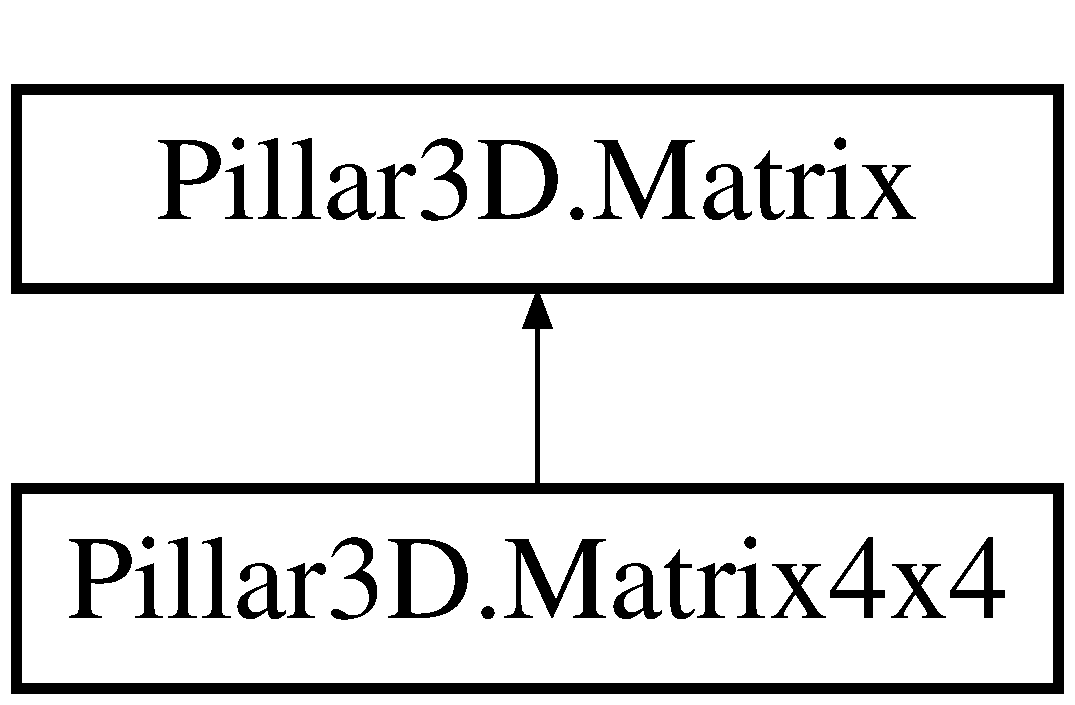
\includegraphics[height=2.000000cm]{class_pillar3_d_1_1_matrix4x4}
\end{center}
\end{figure}
\subsection*{Public Member Functions}
\begin{DoxyCompactItemize}
\item 
\mbox{\Hypertarget{class_pillar3_d_1_1_matrix4x4_ad8b3622dedb3f9932abdf9d47d51de82}\label{class_pillar3_d_1_1_matrix4x4_ad8b3622dedb3f9932abdf9d47d51de82}} 
{\bfseries Matrix4x4} (float\mbox{[}$\,$\mbox{]}\mbox{[}$\,$\mbox{]} initial\+Values)
\item 
\mbox{\Hypertarget{class_pillar3_d_1_1_matrix4x4_a39c8563032213a6f5e77a09eef68d04b}\label{class_pillar3_d_1_1_matrix4x4_a39c8563032213a6f5e77a09eef68d04b}} 
new \hyperlink{class_pillar3_d_1_1_vector4}{Vector4} {\bfseries Get\+Column} (int column)
\item 
\mbox{\Hypertarget{class_pillar3_d_1_1_matrix4x4_a3eb437ba9b70c86161c68e71f7bd95f2}\label{class_pillar3_d_1_1_matrix4x4_a3eb437ba9b70c86161c68e71f7bd95f2}} 
new \hyperlink{class_pillar3_d_1_1_vector4}{Vector4} {\bfseries Get\+Row} (int row)
\item 
\mbox{\Hypertarget{class_pillar3_d_1_1_matrix4x4_a81e5dcd34344bb209183ffba3f856c8d}\label{class_pillar3_d_1_1_matrix4x4_a81e5dcd34344bb209183ffba3f856c8d}} 
void {\bfseries Set\+Column} (int column, \hyperlink{class_pillar3_d_1_1_vector4}{Vector4} values)
\item 
\mbox{\Hypertarget{class_pillar3_d_1_1_matrix4x4_ac2b8f2fb4979b96059f0869f4c86ff39}\label{class_pillar3_d_1_1_matrix4x4_ac2b8f2fb4979b96059f0869f4c86ff39}} 
void {\bfseries Set\+Row} (int row, \hyperlink{class_pillar3_d_1_1_vector4}{Vector4} values)
\end{DoxyCompactItemize}
\subsection*{Static Public Member Functions}
\begin{DoxyCompactItemize}
\item 
\mbox{\Hypertarget{class_pillar3_d_1_1_matrix4x4_a73c342bee53918b131125ebf3f9ae959}\label{class_pillar3_d_1_1_matrix4x4_a73c342bee53918b131125ebf3f9ae959}} 
static \hyperlink{class_pillar3_d_1_1_matrix4x4}{Matrix4x4} {\bfseries T\+RS} (\hyperlink{class_pillar3_d_1_1_vector3}{Vector3} p, \hyperlink{class_pillar3_d_1_1_vector3}{Vector3} r, \hyperlink{class_pillar3_d_1_1_vector3}{Vector3} s)
\item 
\mbox{\Hypertarget{class_pillar3_d_1_1_matrix4x4_abc63327bd6ff4c432b84ca59b8cf05bf}\label{class_pillar3_d_1_1_matrix4x4_abc63327bd6ff4c432b84ca59b8cf05bf}} 
static \hyperlink{class_pillar3_d_1_1_matrix4x4}{Matrix4x4} {\bfseries Translate} (\hyperlink{class_pillar3_d_1_1_vector3}{Vector3} p)
\item 
\mbox{\Hypertarget{class_pillar3_d_1_1_matrix4x4_a211bfd081ec7c8bd2d38a47179696dba}\label{class_pillar3_d_1_1_matrix4x4_a211bfd081ec7c8bd2d38a47179696dba}} 
static \hyperlink{class_pillar3_d_1_1_matrix4x4}{Matrix4x4} {\bfseries Scale} (\hyperlink{class_pillar3_d_1_1_vector3}{Vector3} s)
\item 
\mbox{\Hypertarget{class_pillar3_d_1_1_matrix4x4_a65de40c4ca95d8a724af0dee8a6a2bae}\label{class_pillar3_d_1_1_matrix4x4_a65de40c4ca95d8a724af0dee8a6a2bae}} 
static \hyperlink{class_pillar3_d_1_1_matrix4x4}{Matrix4x4} {\bfseries Rotate} (\hyperlink{class_pillar3_d_1_1_vector3}{Vector3} r)
\end{DoxyCompactItemize}
\subsection*{Additional Inherited Members}


The documentation for this class was generated from the following file\+:\begin{DoxyCompactItemize}
\item 
C\+:/\+Users/gaben/\+Documents/\+Visual Studio 2015/\+Projects/\+Pillar/\+Pillar/\+Internal/Matrix.\+cs\end{DoxyCompactItemize}

\hypertarget{class_pillar3_d_1_1_pillar_behaviour}{}\section{Pillar3\+D.\+Pillar\+Behaviour Class Reference}
\label{class_pillar3_d_1_1_pillar_behaviour}\index{Pillar3\+D.\+Pillar\+Behaviour@{Pillar3\+D.\+Pillar\+Behaviour}}
Inheritance diagram for Pillar3\+D.\+Pillar\+Behaviour\+:\begin{figure}[H]
\begin{center}
\leavevmode
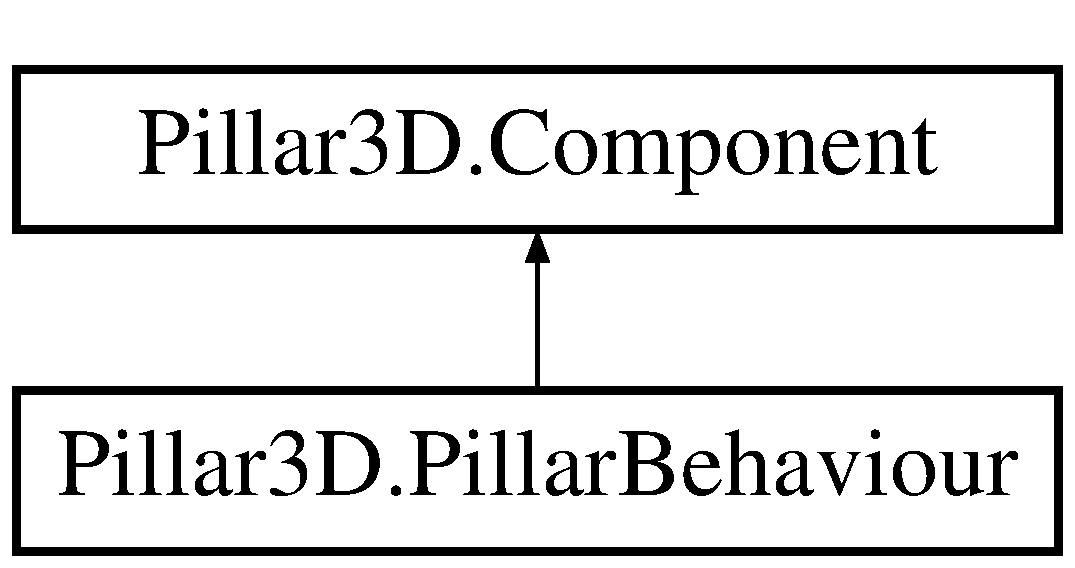
\includegraphics[height=2.000000cm]{class_pillar3_d_1_1_pillar_behaviour}
\end{center}
\end{figure}
\subsection*{Public Member Functions}
\begin{DoxyCompactItemize}
\item 
\mbox{\Hypertarget{class_pillar3_d_1_1_pillar_behaviour_acef99bf3d04dc732634e9421d2753951}\label{class_pillar3_d_1_1_pillar_behaviour_acef99bf3d04dc732634e9421d2753951}} 
abstract void {\bfseries Start} ()
\item 
\mbox{\Hypertarget{class_pillar3_d_1_1_pillar_behaviour_a95e4d79c0e81bb2fbb672b36efcde868}\label{class_pillar3_d_1_1_pillar_behaviour_a95e4d79c0e81bb2fbb672b36efcde868}} 
new abstract void {\bfseries Update} ()
\end{DoxyCompactItemize}
\subsection*{Public Attributes}
\begin{DoxyCompactItemize}
\item 
\mbox{\Hypertarget{class_pillar3_d_1_1_pillar_behaviour_ae80f907c2796c63c4834b866b8468868}\label{class_pillar3_d_1_1_pillar_behaviour_ae80f907c2796c63c4834b866b8468868}} 
bool {\bfseries Enabled}
\end{DoxyCompactItemize}
\subsection*{Additional Inherited Members}


The documentation for this class was generated from the following file\+:\begin{DoxyCompactItemize}
\item 
C\+:/\+Users/gaben/\+Documents/\+Visual Studio 2015/\+Projects/\+Pillar/\+Pillar/\+Internal/Pillar\+Behaviour.\+cs\end{DoxyCompactItemize}

\hypertarget{class_pillar3_d_1_1_quaternion}{}\section{Pillar3\+D.\+Quaternion Class Reference}
\label{class_pillar3_d_1_1_quaternion}\index{Pillar3\+D.\+Quaternion@{Pillar3\+D.\+Quaternion}}
\subsection*{Public Member Functions}
\begin{DoxyCompactItemize}
\item 
\mbox{\Hypertarget{class_pillar3_d_1_1_quaternion_ae31516efc345bbc4ccbaf8c00348e5de}\label{class_pillar3_d_1_1_quaternion_ae31516efc345bbc4ccbaf8c00348e5de}} 
{\bfseries Quaternion} (float x, float y, float z, float w)
\item 
\hyperlink{class_pillar3_d_1_1_quaternion_a82aed3ea7cf7302ebb89d33e45941413}{Quaternion} (\hyperlink{class_pillar3_d_1_1_vector3}{Vector3} Angles)
\begin{DoxyCompactList}\small\item\em Angles is xyz on a unit sphere \end{DoxyCompactList}\item 
\hyperlink{class_pillar3_d_1_1_vector3}{Vector3} \hyperlink{class_pillar3_d_1_1_quaternion_aba7fc95eb3ab95f2ca51d4a205c798db}{To\+Angles} ()
\begin{DoxyCompactList}\small\item\em Converts to xyz on a unit sphere \end{DoxyCompactList}\item 
\mbox{\Hypertarget{class_pillar3_d_1_1_quaternion_aeb011cb05aa967ba639e53234ab74054}\label{class_pillar3_d_1_1_quaternion_aeb011cb05aa967ba639e53234ab74054}} 
\hyperlink{class_pillar3_d_1_1_quaternion}{Quaternion} {\bfseries Look\+Rotation} (\hyperlink{class_pillar3_d_1_1_vector3}{Vector3} forward)
\item 
\mbox{\Hypertarget{class_pillar3_d_1_1_quaternion_a5184e9984a322ed6acc53da1954d10f2}\label{class_pillar3_d_1_1_quaternion_a5184e9984a322ed6acc53da1954d10f2}} 
\hyperlink{class_pillar3_d_1_1_quaternion}{Quaternion} {\bfseries Look\+Rotation} (\hyperlink{class_pillar3_d_1_1_vector3}{Vector3} forward, \hyperlink{class_pillar3_d_1_1_vector3}{Vector3} up)
\end{DoxyCompactItemize}
\subsection*{Static Public Member Functions}
\begin{DoxyCompactItemize}
\item 
\mbox{\Hypertarget{class_pillar3_d_1_1_quaternion_a55910a158e22f9b1eb91bfc63358ba9a}\label{class_pillar3_d_1_1_quaternion_a55910a158e22f9b1eb91bfc63358ba9a}} 
static \hyperlink{class_pillar3_d_1_1_quaternion}{Quaternion} {\bfseries operator$\ast$} (\hyperlink{class_pillar3_d_1_1_quaternion}{Quaternion} a, \hyperlink{class_pillar3_d_1_1_quaternion}{Quaternion} b)
\item 
\mbox{\Hypertarget{class_pillar3_d_1_1_quaternion_a4aad30009497a99cc92be7803bdb787a}\label{class_pillar3_d_1_1_quaternion_a4aad30009497a99cc92be7803bdb787a}} 
static \hyperlink{class_pillar3_d_1_1_vector3}{Vector3} {\bfseries operator$\ast$} (\hyperlink{class_pillar3_d_1_1_quaternion}{Quaternion} lhs, \hyperlink{class_pillar3_d_1_1_vector3}{Vector3} rhs)
\item 
\mbox{\Hypertarget{class_pillar3_d_1_1_quaternion_af1536058adc5b68a327102d5f20f61a4}\label{class_pillar3_d_1_1_quaternion_af1536058adc5b68a327102d5f20f61a4}} 
static \hyperlink{class_pillar3_d_1_1_vector3}{Vector3} {\bfseries operator$\ast$} (\hyperlink{class_pillar3_d_1_1_vector3}{Vector3} lhs, \hyperlink{class_pillar3_d_1_1_quaternion}{Quaternion} rhs)
\item 
\mbox{\Hypertarget{class_pillar3_d_1_1_quaternion_ac659977c8ac4a053df26033117f0cbcb}\label{class_pillar3_d_1_1_quaternion_ac659977c8ac4a053df26033117f0cbcb}} 
static {\bfseries operator Matrix} (\hyperlink{class_pillar3_d_1_1_quaternion}{Quaternion} q)
\end{DoxyCompactItemize}
\subsection*{Public Attributes}
\begin{DoxyCompactItemize}
\item 
\mbox{\Hypertarget{class_pillar3_d_1_1_quaternion_a7437a39c5debcbdd2f97812eadf664aa}\label{class_pillar3_d_1_1_quaternion_a7437a39c5debcbdd2f97812eadf664aa}} 
float {\bfseries x}
\end{DoxyCompactItemize}
\subsection*{Properties}
\begin{DoxyCompactItemize}
\item 
\mbox{\Hypertarget{class_pillar3_d_1_1_quaternion_a9e0a2596ecdb60e40faf6580dd1ee0c2}\label{class_pillar3_d_1_1_quaternion_a9e0a2596ecdb60e40faf6580dd1ee0c2}} 
static \hyperlink{class_pillar3_d_1_1_quaternion}{Quaternion} {\bfseries Identity}\hspace{0.3cm}{\ttfamily  \mbox{[}get\mbox{]}}
\end{DoxyCompactItemize}


\subsection{Constructor \& Destructor Documentation}
\mbox{\Hypertarget{class_pillar3_d_1_1_quaternion_a82aed3ea7cf7302ebb89d33e45941413}\label{class_pillar3_d_1_1_quaternion_a82aed3ea7cf7302ebb89d33e45941413}} 
\index{Pillar3\+D\+::\+Quaternion@{Pillar3\+D\+::\+Quaternion}!Quaternion@{Quaternion}}
\index{Quaternion@{Quaternion}!Pillar3\+D\+::\+Quaternion@{Pillar3\+D\+::\+Quaternion}}
\subsubsection{\texorpdfstring{Quaternion()}{Quaternion()}}
{\footnotesize\ttfamily Pillar3\+D.\+Quaternion.\+Quaternion (\begin{DoxyParamCaption}\item[{\hyperlink{class_pillar3_d_1_1_vector3}{Vector3}}]{Angles }\end{DoxyParamCaption})}



Angles is xyz on a unit sphere 


\begin{DoxyParams}{Parameters}
{\em Angles} & \\
\hline
\end{DoxyParams}


\subsection{Member Function Documentation}
\mbox{\Hypertarget{class_pillar3_d_1_1_quaternion_aba7fc95eb3ab95f2ca51d4a205c798db}\label{class_pillar3_d_1_1_quaternion_aba7fc95eb3ab95f2ca51d4a205c798db}} 
\index{Pillar3\+D\+::\+Quaternion@{Pillar3\+D\+::\+Quaternion}!To\+Angles@{To\+Angles}}
\index{To\+Angles@{To\+Angles}!Pillar3\+D\+::\+Quaternion@{Pillar3\+D\+::\+Quaternion}}
\subsubsection{\texorpdfstring{To\+Angles()}{ToAngles()}}
{\footnotesize\ttfamily \hyperlink{class_pillar3_d_1_1_vector3}{Vector3} Pillar3\+D.\+Quaternion.\+To\+Angles (\begin{DoxyParamCaption}{ }\end{DoxyParamCaption})}



Converts to xyz on a unit sphere 

\begin{DoxyReturn}{Returns}

\end{DoxyReturn}


The documentation for this class was generated from the following file\+:\begin{DoxyCompactItemize}
\item 
C\+:/\+Users/gaben/\+Documents/\+Visual Studio 2015/\+Projects/\+Pillar/\+Pillar/\+Internal/Quaternion.\+cs\end{DoxyCompactItemize}

\hypertarget{class_pillar3_d_1_1_rails}{}\section{Pillar3\+D.\+Rails Class Reference}
\label{class_pillar3_d_1_1_rails}\index{Pillar3\+D.\+Rails@{Pillar3\+D.\+Rails}}
\subsection*{Static Public Member Functions}
\begin{DoxyCompactItemize}
\item 
\mbox{\Hypertarget{class_pillar3_d_1_1_rails_aa918313a95451095b7290da48f7a02c6}\label{class_pillar3_d_1_1_rails_aa918313a95451095b7290da48f7a02c6}} 
static void {\bfseries Exit} ()
\item 
\mbox{\Hypertarget{class_pillar3_d_1_1_rails_ad9bc7982aa9ddfeed3f87ef86c7e732e}\label{class_pillar3_d_1_1_rails_ad9bc7982aa9ddfeed3f87ef86c7e732e}} 
static void {\bfseries Change\+Level} (\hyperlink{class_pillar3_d_1_1_entity}{Entity} entity, \hyperlink{class_pillar3_d_1_1_level}{Level} new\+Level)
\end{DoxyCompactItemize}
\subsection*{Public Attributes}
\begin{DoxyCompactItemize}
\item 
\mbox{\Hypertarget{class_pillar3_d_1_1_rails_a1e2db16fc0eb4a1cc759ea54fb4f36f3}\label{class_pillar3_d_1_1_rails_a1e2db16fc0eb4a1cc759ea54fb4f36f3}} 
Action {\bfseries Initialize}
\item 
\mbox{\Hypertarget{class_pillar3_d_1_1_rails_a111399e1129e557f099c5bd3e09b7df2}\label{class_pillar3_d_1_1_rails_a111399e1129e557f099c5bd3e09b7df2}} 
bool {\bfseries Paused} = false
\end{DoxyCompactItemize}
\subsection*{Static Public Attributes}
\begin{DoxyCompactItemize}
\item 
\mbox{\Hypertarget{class_pillar3_d_1_1_rails_a531b02c1daf778ca5a0ad2fbe11001c5}\label{class_pillar3_d_1_1_rails_a531b02c1daf778ca5a0ad2fbe11001c5}} 
static bool {\bfseries Global\+Pause} = false
\item 
\mbox{\Hypertarget{class_pillar3_d_1_1_rails_aff2abff15d3bb346dae537755ad57688}\label{class_pillar3_d_1_1_rails_aff2abff15d3bb346dae537755ad57688}} 
static Action {\bfseries Global\+Update}
\end{DoxyCompactItemize}


The documentation for this class was generated from the following file\+:\begin{DoxyCompactItemize}
\item 
C\+:/\+Users/gaben/\+Documents/\+Visual Studio 2015/\+Projects/\+Pillar/\+Pillar/\+Internal/Program.\+cs\end{DoxyCompactItemize}

\hypertarget{class_pillar3_d_1_1_routine_runner}{}\section{Pillar3\+D.\+Routine\+Runner Class Reference}
\label{class_pillar3_d_1_1_routine_runner}\index{Pillar3\+D.\+Routine\+Runner@{Pillar3\+D.\+Routine\+Runner}}
\subsection*{Public Member Functions}
\begin{DoxyCompactItemize}
\item 
\mbox{\Hypertarget{class_pillar3_d_1_1_routine_runner_ab3443046a8444994ab5ac1de1411c9a8}\label{class_pillar3_d_1_1_routine_runner_ab3443046a8444994ab5ac1de1411c9a8}} 
void {\bfseries Frame} ()
\end{DoxyCompactItemize}
\subsection*{Static Public Member Functions}
\begin{DoxyCompactItemize}
\item 
\mbox{\Hypertarget{class_pillar3_d_1_1_routine_runner_a99b2e40303c3b01d61f4c189ccbdd173}\label{class_pillar3_d_1_1_routine_runner_a99b2e40303c3b01d61f4c189ccbdd173}} 
static void {\bfseries Run\+Routine} (I\+Enumerator$<$ \hyperlink{class_pillar3_d_1_1_yield_instruction}{Yield\+Instruction} $>$ routine)
\end{DoxyCompactItemize}


The documentation for this class was generated from the following file\+:\begin{DoxyCompactItemize}
\item 
C\+:/\+Users/gaben/\+Documents/\+Visual Studio 2015/\+Projects/\+Pillar/\+Pillar/\+Internal/Yield\+Instruction.\+cs\end{DoxyCompactItemize}

\hypertarget{class_sample_component}{}\section{Sample\+Component Class Reference}
\label{class_sample_component}\index{Sample\+Component@{Sample\+Component}}
Inheritance diagram for Sample\+Component\+:\begin{figure}[H]
\begin{center}
\leavevmode
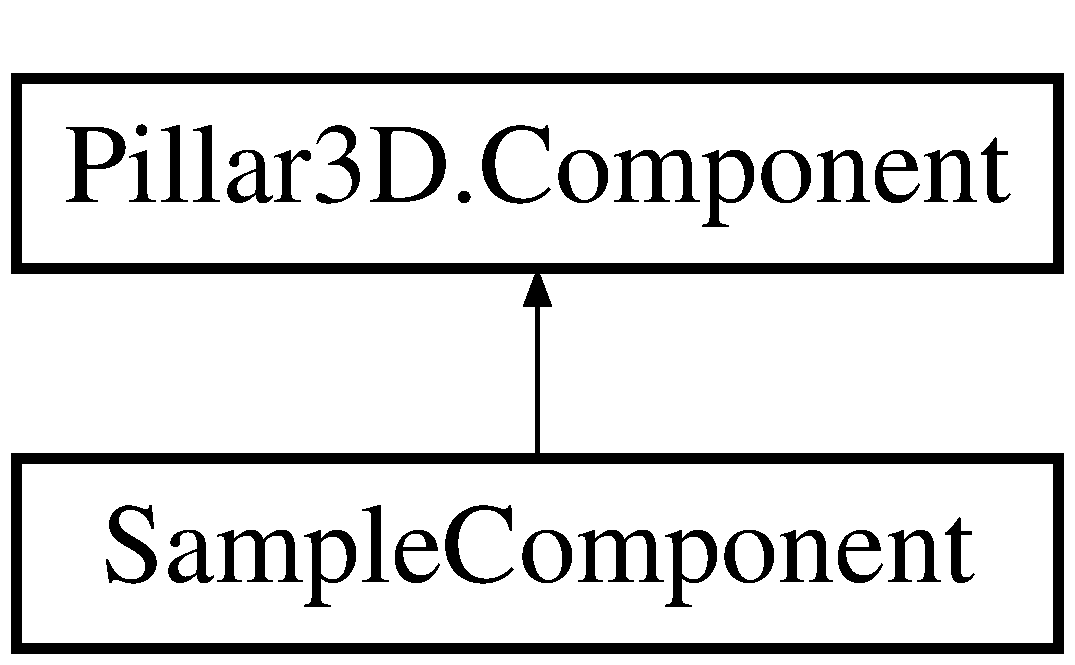
\includegraphics[height=2.000000cm]{class_sample_component}
\end{center}
\end{figure}
\subsection*{Public Member Functions}
\begin{DoxyCompactItemize}
\item 
\mbox{\Hypertarget{class_sample_component_ad314fb7299417e9eee4955f5d11c1b2e}\label{class_sample_component_ad314fb7299417e9eee4955f5d11c1b2e}} 
new void {\bfseries Update} ()
\end{DoxyCompactItemize}
\subsection*{Additional Inherited Members}


The documentation for this class was generated from the following file\+:\begin{DoxyCompactItemize}
\item 
C\+:/\+Users/gaben/\+Documents/\+Visual Studio 2015/\+Projects/\+Pillar/\+Pillar/\+Project Assets/Sample\+Component.\+cs\end{DoxyCompactItemize}

\hypertarget{class_pillar3_d_1_1_settings}{}\section{Pillar3\+D.\+Settings Class Reference}
\label{class_pillar3_d_1_1_settings}\index{Pillar3\+D.\+Settings@{Pillar3\+D.\+Settings}}
\subsection*{Static Public Attributes}
\begin{DoxyCompactItemize}
\item 
\mbox{\Hypertarget{class_pillar3_d_1_1_settings_a7a6cee261459620721ab11476e6a154b}\label{class_pillar3_d_1_1_settings_a7a6cee261459620721ab11476e6a154b}} 
static Sync\+State {\bfseries V\+Sync} = Sync\+State.\+Sync\+Threads
\end{DoxyCompactItemize}


The documentation for this class was generated from the following file\+:\begin{DoxyCompactItemize}
\item 
C\+:/\+Users/gaben/\+Documents/\+Visual Studio 2015/\+Projects/\+Pillar/\+Pillar/\+Internal/Settings.\+cs\end{DoxyCompactItemize}

\hypertarget{class_pillar3_d_1_1_smart_cache}{}\section{Pillar3\+D.\+Smart\+Cache$<$ T $>$ Class Template Reference}
\label{class_pillar3_d_1_1_smart_cache}\index{Pillar3\+D.\+Smart\+Cache$<$ T $>$@{Pillar3\+D.\+Smart\+Cache$<$ T $>$}}
\subsection*{Public Member Functions}
\begin{DoxyCompactItemize}
\item 
\mbox{\Hypertarget{class_pillar3_d_1_1_smart_cache_aa429f916ecf2c31615adbb209f00e5f6}\label{class_pillar3_d_1_1_smart_cache_aa429f916ecf2c31615adbb209f00e5f6}} 
{\bfseries Smart\+Cache} (Func$<$ T $>$ Calculator, T initial\+Value)
\item 
\mbox{\Hypertarget{class_pillar3_d_1_1_smart_cache_af86e2b3e94b309d76cfcc3ba9c8250b6}\label{class_pillar3_d_1_1_smart_cache_af86e2b3e94b309d76cfcc3ba9c8250b6}} 
void {\bfseries Dirty} ()
\end{DoxyCompactItemize}
\subsection*{Properties}
\begin{DoxyCompactItemize}
\item 
\mbox{\Hypertarget{class_pillar3_d_1_1_smart_cache_a5bc41dc327077e56feb07d08a045659f}\label{class_pillar3_d_1_1_smart_cache_a5bc41dc327077e56feb07d08a045659f}} 
T {\bfseries Value}\hspace{0.3cm}{\ttfamily  \mbox{[}get, set\mbox{]}}
\end{DoxyCompactItemize}


The documentation for this class was generated from the following file\+:\begin{DoxyCompactItemize}
\item 
C\+:/\+Users/gaben/\+Documents/\+Visual Studio 2015/\+Projects/\+Pillar/\+Pillar/\+Internal/Utilities.\+cs\end{DoxyCompactItemize}

\hypertarget{class_test_class}{}\section{Test\+Class Class Reference}
\label{class_test_class}\index{Test\+Class@{Test\+Class}}
\subsection*{Public Member Functions}
\begin{DoxyCompactItemize}
\item 
\mbox{\Hypertarget{class_test_class_a898cc2b04d72c863aba09740f8843807}\label{class_test_class_a898cc2b04d72c863aba09740f8843807}} 
I\+Enumerator$<$ \hyperlink{class_pillar3_d_1_1_yield_instruction}{Yield\+Instruction} $>$ {\bfseries Example\+Routine} ()
\end{DoxyCompactItemize}


The documentation for this class was generated from the following file\+:\begin{DoxyCompactItemize}
\item 
C\+:/\+Users/gaben/\+Documents/\+Visual Studio 2015/\+Projects/\+Pillar/\+Pillar/\+Project Assets/Test\+Class.\+cs\end{DoxyCompactItemize}

\hypertarget{class_pillar3_d_1_1_thread_manager}{}\section{Pillar3\+D.\+Thread\+Manager Class Reference}
\label{class_pillar3_d_1_1_thread_manager}\index{Pillar3\+D.\+Thread\+Manager@{Pillar3\+D.\+Thread\+Manager}}
\subsection*{Static Public Member Functions}
\begin{DoxyCompactItemize}
\item 
\mbox{\Hypertarget{class_pillar3_d_1_1_thread_manager_a63db83e5522df03991d1a8185fd52af0}\label{class_pillar3_d_1_1_thread_manager_a63db83e5522df03991d1a8185fd52af0}} 
static void {\bfseries Add\+Level} (\hyperlink{class_pillar3_d_1_1_level}{Level} level)
\item 
\mbox{\Hypertarget{class_pillar3_d_1_1_thread_manager_a710bc7fb00c6ec5c02cce9e3ffd167fb}\label{class_pillar3_d_1_1_thread_manager_a710bc7fb00c6ec5c02cce9e3ffd167fb}} 
static void {\bfseries Remove\+Level} (\hyperlink{class_pillar3_d_1_1_level}{Level} level)
\item 
\mbox{\Hypertarget{class_pillar3_d_1_1_thread_manager_a9a202245f3cd86a1d4a114f5a26b7219}\label{class_pillar3_d_1_1_thread_manager_a9a202245f3cd86a1d4a114f5a26b7219}} 
static bool {\bfseries Get\+Threads\+Idle} ()
\item 
\mbox{\Hypertarget{class_pillar3_d_1_1_thread_manager_a05e5b3644524692bcc2f6e9524260e1b}\label{class_pillar3_d_1_1_thread_manager_a05e5b3644524692bcc2f6e9524260e1b}} 
static bool {\bfseries Frame} ()
\end{DoxyCompactItemize}


The documentation for this class was generated from the following file\+:\begin{DoxyCompactItemize}
\item 
C\+:/\+Users/gaben/\+Documents/\+Visual Studio 2015/\+Projects/\+Pillar/\+Pillar/\+Internal/Program.\+cs\end{DoxyCompactItemize}

\hypertarget{class_pillar3_d_1_1_time}{}\section{Pillar3\+D.\+Time Class Reference}
\label{class_pillar3_d_1_1_time}\index{Pillar3\+D.\+Time@{Pillar3\+D.\+Time}}
\subsection*{Public Member Functions}
\begin{DoxyCompactItemize}
\item 
\mbox{\Hypertarget{class_pillar3_d_1_1_time_a10919378ee5b28a69a8b8b1452fe87e1}\label{class_pillar3_d_1_1_time_a10919378ee5b28a69a8b8b1452fe87e1}} 
void {\bfseries Frame} ()
\end{DoxyCompactItemize}
\subsection*{Static Public Attributes}
\begin{DoxyCompactItemize}
\item 
\mbox{\Hypertarget{class_pillar3_d_1_1_time_a933d9a77b8cdb43ccd08c4eb8a1462df}\label{class_pillar3_d_1_1_time_a933d9a77b8cdb43ccd08c4eb8a1462df}} 
static float {\bfseries Time\+Scale}
\item 
\mbox{\Hypertarget{class_pillar3_d_1_1_time_acbd9879ea141bec6ed6219e248686b67}\label{class_pillar3_d_1_1_time_acbd9879ea141bec6ed6219e248686b67}} 
static int {\bfseries Sample\+Count}
\end{DoxyCompactItemize}
\subsection*{Properties}
\begin{DoxyCompactItemize}
\item 
\mbox{\Hypertarget{class_pillar3_d_1_1_time_a601a80c9e850076707b071dfa7c08a21}\label{class_pillar3_d_1_1_time_a601a80c9e850076707b071dfa7c08a21}} 
static float {\bfseries Delta\+Time}\hspace{0.3cm}{\ttfamily  \mbox{[}get\mbox{]}}
\item 
\mbox{\Hypertarget{class_pillar3_d_1_1_time_a750754af29660f91ec00ac9a9110e85f}\label{class_pillar3_d_1_1_time_a750754af29660f91ec00ac9a9110e85f}} 
static float {\bfseries Real\+Time}\hspace{0.3cm}{\ttfamily  \mbox{[}get\mbox{]}}
\item 
\mbox{\Hypertarget{class_pillar3_d_1_1_time_afac9966351eb52070bb2658d3d7c2f84}\label{class_pillar3_d_1_1_time_afac9966351eb52070bb2658d3d7c2f84}} 
static float {\bfseries Scaled\+Time}\hspace{0.3cm}{\ttfamily  \mbox{[}get\mbox{]}}
\item 
\mbox{\Hypertarget{class_pillar3_d_1_1_time_a73c7fcefe5ebbdbfbb410628d3d1e3a7}\label{class_pillar3_d_1_1_time_a73c7fcefe5ebbdbfbb410628d3d1e3a7}} 
static long {\bfseries Frame\+Count}\hspace{0.3cm}{\ttfamily  \mbox{[}get\mbox{]}}
\item 
\mbox{\Hypertarget{class_pillar3_d_1_1_time_aebb0c309c86c95ef5e4ec86d99468a5b}\label{class_pillar3_d_1_1_time_aebb0c309c86c95ef5e4ec86d99468a5b}} 
static float {\bfseries Smooth\+Delta\+Time}\hspace{0.3cm}{\ttfamily  \mbox{[}get\mbox{]}}
\end{DoxyCompactItemize}


The documentation for this class was generated from the following file\+:\begin{DoxyCompactItemize}
\item 
C\+:/\+Users/gaben/\+Documents/\+Visual Studio 2015/\+Projects/\+Pillar/\+Pillar/\+Internal/Time.\+cs\end{DoxyCompactItemize}

\hypertarget{class_pillar3_d_1_1_internal_1_1_tracked_thread}{}\section{Pillar3\+D.\+Internal.\+Tracked\+Thread Class Reference}
\label{class_pillar3_d_1_1_internal_1_1_tracked_thread}\index{Pillar3\+D.\+Internal.\+Tracked\+Thread@{Pillar3\+D.\+Internal.\+Tracked\+Thread}}
\subsection*{Public Member Functions}
\begin{DoxyCompactItemize}
\item 
\mbox{\Hypertarget{class_pillar3_d_1_1_internal_1_1_tracked_thread_af8e659f6beb78cf418b629170bee6b5f}\label{class_pillar3_d_1_1_internal_1_1_tracked_thread_af8e659f6beb78cf418b629170bee6b5f}} 
{\bfseries Tracked\+Thread} (\hyperlink{class_pillar3_d_1_1_level}{Level} level)
\item 
\mbox{\Hypertarget{class_pillar3_d_1_1_internal_1_1_tracked_thread_ab471add59a8e24860d57a626315ffb82}\label{class_pillar3_d_1_1_internal_1_1_tracked_thread_ab471add59a8e24860d57a626315ffb82}} 
void {\bfseries Add\+Level} (\hyperlink{class_pillar3_d_1_1_level}{Level} level)
\item 
\mbox{\Hypertarget{class_pillar3_d_1_1_internal_1_1_tracked_thread_aab614d6a10b824b541ac043be6bc59ff}\label{class_pillar3_d_1_1_internal_1_1_tracked_thread_aab614d6a10b824b541ac043be6bc59ff}} 
void {\bfseries Frame} ()
\end{DoxyCompactItemize}
\subsection*{Public Attributes}
\begin{DoxyCompactItemize}
\item 
\mbox{\Hypertarget{class_pillar3_d_1_1_internal_1_1_tracked_thread_a84fc011ef6591e83bb8dfded470613e3}\label{class_pillar3_d_1_1_internal_1_1_tracked_thread_a84fc011ef6591e83bb8dfded470613e3}} 
int {\bfseries Stress} = 0
\item 
\mbox{\Hypertarget{class_pillar3_d_1_1_internal_1_1_tracked_thread_afd1496fc69ff185beac724a469579eaa}\label{class_pillar3_d_1_1_internal_1_1_tracked_thread_afd1496fc69ff185beac724a469579eaa}} 
List$<$ \hyperlink{class_pillar3_d_1_1_level}{Level} $>$ {\bfseries Levels} = new List$<$\hyperlink{class_pillar3_d_1_1_level}{Level}$>$()
\end{DoxyCompactItemize}


The documentation for this class was generated from the following file\+:\begin{DoxyCompactItemize}
\item 
C\+:/\+Users/gaben/\+Documents/\+Visual Studio 2015/\+Projects/\+Pillar/\+Pillar/\+Internal/Tracked\+Thread.\+cs\end{DoxyCompactItemize}

\hypertarget{class_pillar3_d_1_1_transform}{}\section{Pillar3\+D.\+Transform Class Reference}
\label{class_pillar3_d_1_1_transform}\index{Pillar3\+D.\+Transform@{Pillar3\+D.\+Transform}}
Inheritance diagram for Pillar3\+D.\+Transform\+:\begin{figure}[H]
\begin{center}
\leavevmode
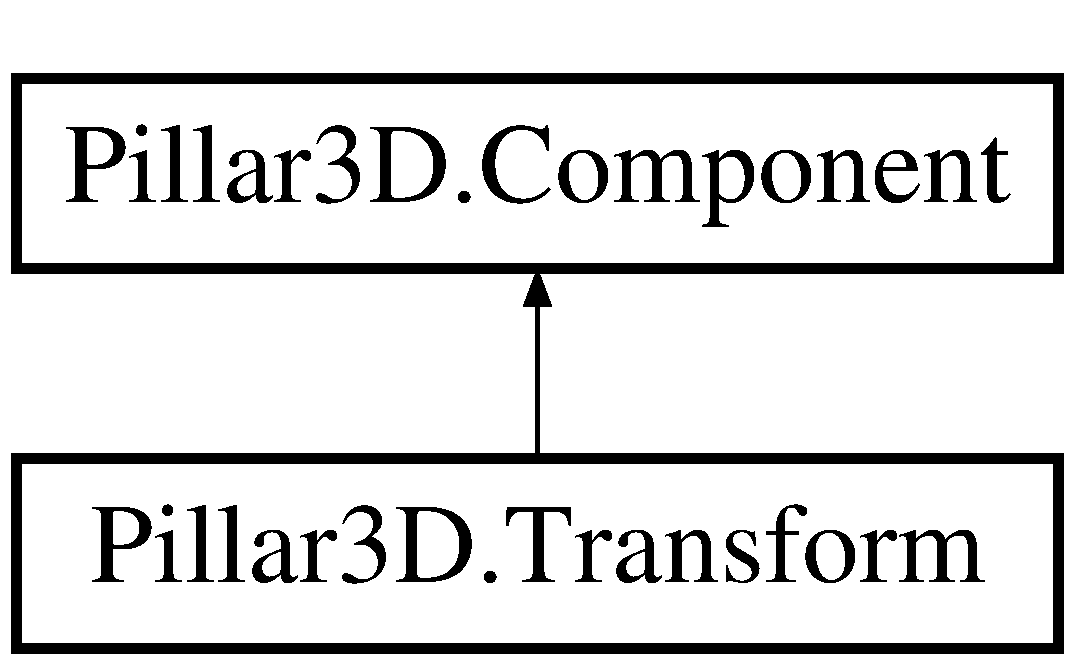
\includegraphics[height=2.000000cm]{class_pillar3_d_1_1_transform}
\end{center}
\end{figure}
\subsection*{Public Member Functions}
\begin{DoxyCompactItemize}
\item 
\mbox{\Hypertarget{class_pillar3_d_1_1_transform_a0b6d30af9034cefa3a508fbc07ec1575}\label{class_pillar3_d_1_1_transform_a0b6d30af9034cefa3a508fbc07ec1575}} 
override void {\bfseries On\+Component\+Added} ()
\end{DoxyCompactItemize}
\subsection*{Public Attributes}
\begin{DoxyCompactItemize}
\item 
\mbox{\Hypertarget{class_pillar3_d_1_1_transform_a9c8f61e79731d3e0c003232529e1e338}\label{class_pillar3_d_1_1_transform_a9c8f61e79731d3e0c003232529e1e338}} 
\hyperlink{class_pillar3_d_1_1_transform}{Transform} {\bfseries parent}
\item 
\mbox{\Hypertarget{class_pillar3_d_1_1_transform_a3d3c7ba18825079d5105ea0445f25faa}\label{class_pillar3_d_1_1_transform_a3d3c7ba18825079d5105ea0445f25faa}} 
Action {\bfseries On\+Transform\+Changed}
\end{DoxyCompactItemize}
\subsection*{Protected Member Functions}
\begin{DoxyCompactItemize}
\item 
\mbox{\Hypertarget{class_pillar3_d_1_1_transform_aa7977f9a5f9270f5c89a7edd97d20042}\label{class_pillar3_d_1_1_transform_aa7977f9a5f9270f5c89a7edd97d20042}} 
void {\bfseries Update\+Children} ()
\item 
\mbox{\Hypertarget{class_pillar3_d_1_1_transform_a30f95c9bbc9e0431bbfe51dfe72b5f46}\label{class_pillar3_d_1_1_transform_a30f95c9bbc9e0431bbfe51dfe72b5f46}} 
void {\bfseries Reparent} ()
\end{DoxyCompactItemize}
\subsection*{Properties}
\begin{DoxyCompactItemize}
\item 
\mbox{\Hypertarget{class_pillar3_d_1_1_transform_a8b02658be952e1ded6862366dc688255}\label{class_pillar3_d_1_1_transform_a8b02658be952e1ded6862366dc688255}} 
\hyperlink{class_pillar3_d_1_1_vector3}{Vector3} {\bfseries Position}\hspace{0.3cm}{\ttfamily  \mbox{[}get, set\mbox{]}}
\item 
\mbox{\Hypertarget{class_pillar3_d_1_1_transform_a79f83ccc5295de3d82c652ae2d266d41}\label{class_pillar3_d_1_1_transform_a79f83ccc5295de3d82c652ae2d266d41}} 
\hyperlink{class_pillar3_d_1_1_vector3}{Vector3} {\bfseries Local\+Position}\hspace{0.3cm}{\ttfamily  \mbox{[}get, set\mbox{]}}
\item 
\mbox{\Hypertarget{class_pillar3_d_1_1_transform_aa66155413ef70fc432926aac718c3a0f}\label{class_pillar3_d_1_1_transform_aa66155413ef70fc432926aac718c3a0f}} 
\hyperlink{class_pillar3_d_1_1_quaternion}{Quaternion} {\bfseries Rotation}\hspace{0.3cm}{\ttfamily  \mbox{[}get, set\mbox{]}}
\item 
\mbox{\Hypertarget{class_pillar3_d_1_1_transform_a7afa852af6c0e0474b958042f2c5a1fb}\label{class_pillar3_d_1_1_transform_a7afa852af6c0e0474b958042f2c5a1fb}} 
\hyperlink{class_pillar3_d_1_1_quaternion}{Quaternion} {\bfseries Local\+Rotation}\hspace{0.3cm}{\ttfamily  \mbox{[}get, set\mbox{]}}
\item 
\mbox{\Hypertarget{class_pillar3_d_1_1_transform_a7f6547c7e5337b35cff885df24378e9a}\label{class_pillar3_d_1_1_transform_a7f6547c7e5337b35cff885df24378e9a}} 
\hyperlink{class_pillar3_d_1_1_vector3}{Vector3} {\bfseries Scale}\hspace{0.3cm}{\ttfamily  \mbox{[}get, set\mbox{]}}
\item 
\mbox{\Hypertarget{class_pillar3_d_1_1_transform_ac59c67249ec0fc49c080a5c92131e169}\label{class_pillar3_d_1_1_transform_ac59c67249ec0fc49c080a5c92131e169}} 
\hyperlink{class_pillar3_d_1_1_vector3}{Vector3} {\bfseries Local\+Scale}\hspace{0.3cm}{\ttfamily  \mbox{[}get, set\mbox{]}}
\end{DoxyCompactItemize}
\subsection*{Additional Inherited Members}


The documentation for this class was generated from the following files\+:\begin{DoxyCompactItemize}
\item 
C\+:/\+Users/gaben/\+Documents/\+Visual Studio 2015/\+Projects/\+Pillar/\+Pillar/\+Internal/L\+Alg\+Transform.\+cs\item 
C\+:/\+Users/gaben/\+Documents/\+Visual Studio 2015/\+Projects/\+Pillar/\+Pillar/\+Internal/Transform.\+cs\end{DoxyCompactItemize}

\hypertarget{class_pillar3_d_1_1_vector2}{}\section{Pillar3\+D.\+Vector2 Class Reference}
\label{class_pillar3_d_1_1_vector2}\index{Pillar3\+D.\+Vector2@{Pillar3\+D.\+Vector2}}
Inheritance diagram for Pillar3\+D.\+Vector2\+:\begin{figure}[H]
\begin{center}
\leavevmode
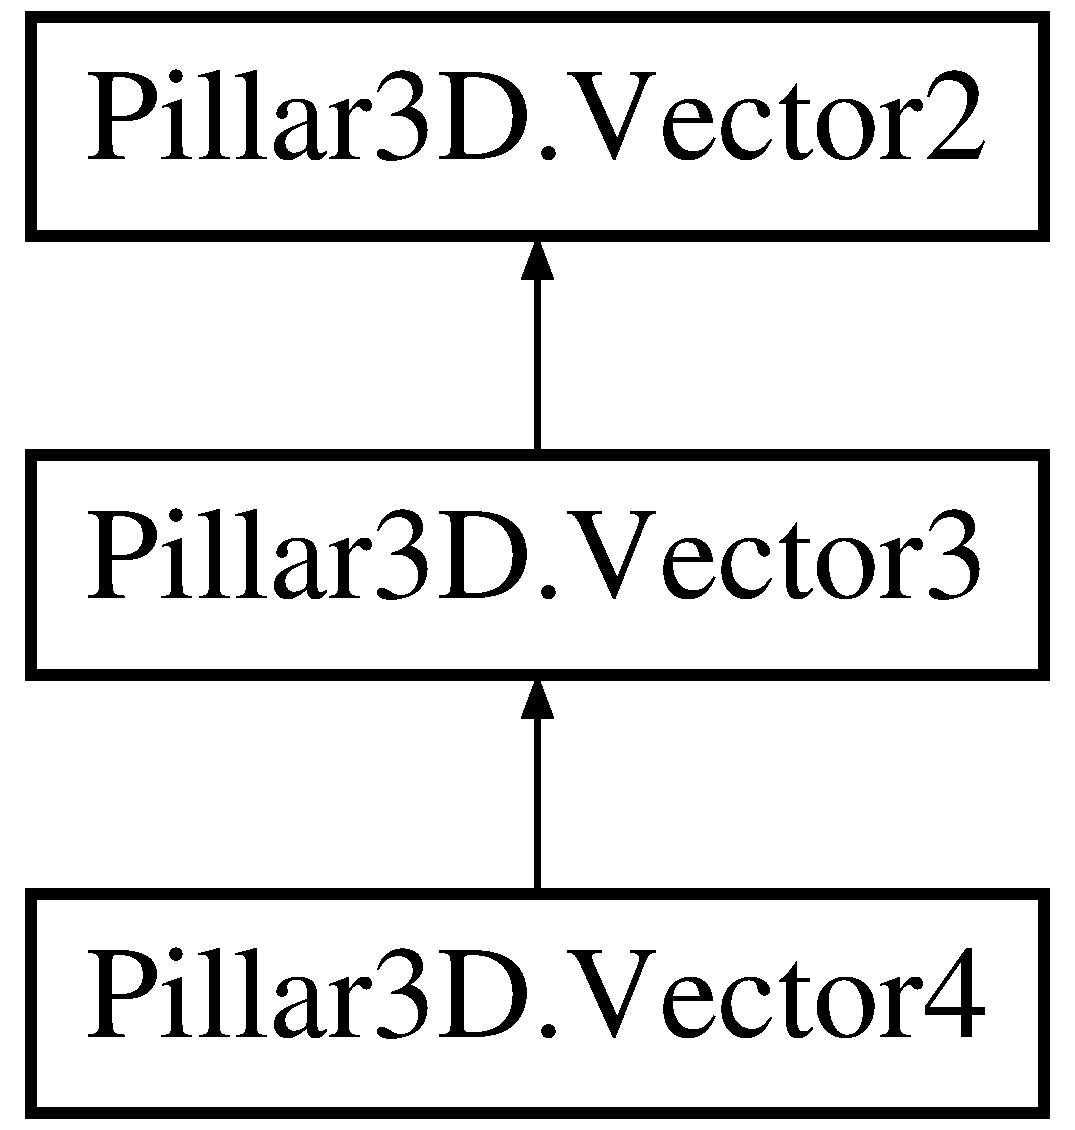
\includegraphics[height=3.000000cm]{class_pillar3_d_1_1_vector2}
\end{center}
\end{figure}
\subsection*{Public Member Functions}
\begin{DoxyCompactItemize}
\item 
\mbox{\Hypertarget{class_pillar3_d_1_1_vector2_abaaf6ec2638337b80154c0cf4ba19e45}\label{class_pillar3_d_1_1_vector2_abaaf6ec2638337b80154c0cf4ba19e45}} 
{\bfseries Vector2} (float x, float y)
\item 
\mbox{\Hypertarget{class_pillar3_d_1_1_vector2_ad5348ad15457aa733e6d87a313de299b}\label{class_pillar3_d_1_1_vector2_ad5348ad15457aa733e6d87a313de299b}} 
{\bfseries Vector2} (\hyperlink{class_pillar3_d_1_1_vector2}{Vector2} original)
\item 
\mbox{\Hypertarget{class_pillar3_d_1_1_vector2_ac12b5df437a5d5a8a91cda9a4d76ac17}\label{class_pillar3_d_1_1_vector2_ac12b5df437a5d5a8a91cda9a4d76ac17}} 
float {\bfseries Magnitude} ()
\item 
\mbox{\Hypertarget{class_pillar3_d_1_1_vector2_a77487bd2b0dfb7060bf2a9a76400f848}\label{class_pillar3_d_1_1_vector2_a77487bd2b0dfb7060bf2a9a76400f848}} 
float {\bfseries Sqr\+Magnitude} ()
\item 
\mbox{\Hypertarget{class_pillar3_d_1_1_vector2_ac9a012cfe0280aa940903ddfc7f9f0a5}\label{class_pillar3_d_1_1_vector2_ac9a012cfe0280aa940903ddfc7f9f0a5}} 
\hyperlink{class_pillar3_d_1_1_vector2}{Vector2} {\bfseries Normalize} ()
\item 
\mbox{\Hypertarget{class_pillar3_d_1_1_vector2_a8624d01486dd3a3ee0f38c3a08a3cc6a}\label{class_pillar3_d_1_1_vector2_a8624d01486dd3a3ee0f38c3a08a3cc6a}} 
\hyperlink{class_pillar3_d_1_1_vector2}{Vector2} {\bfseries Normalized} ()
\item 
\mbox{\Hypertarget{class_pillar3_d_1_1_vector2_a0522c8831f61d887d744faa890cf0c31}\label{class_pillar3_d_1_1_vector2_a0522c8831f61d887d744faa890cf0c31}} 
override string {\bfseries To\+String} ()
\item 
\mbox{\Hypertarget{class_pillar3_d_1_1_vector2_a5863668e2bf329cf661790d53c33976f}\label{class_pillar3_d_1_1_vector2_a5863668e2bf329cf661790d53c33976f}} 
override bool {\bfseries Equals} (object other)
\item 
\mbox{\Hypertarget{class_pillar3_d_1_1_vector2_a19efd9e2a774fd8e5822ec988eb03229}\label{class_pillar3_d_1_1_vector2_a19efd9e2a774fd8e5822ec988eb03229}} 
override int {\bfseries Get\+Hash\+Code} ()
\end{DoxyCompactItemize}
\subsection*{Static Public Member Functions}
\begin{DoxyCompactItemize}
\item 
\mbox{\Hypertarget{class_pillar3_d_1_1_vector2_af351b63df18e9d8f90fb9d4c16594569}\label{class_pillar3_d_1_1_vector2_af351b63df18e9d8f90fb9d4c16594569}} 
static float {\bfseries Dot} (\hyperlink{class_pillar3_d_1_1_vector2}{Vector2} lhs, \hyperlink{class_pillar3_d_1_1_vector2}{Vector2} rhs)
\item 
\mbox{\Hypertarget{class_pillar3_d_1_1_vector2_a70521028b7977623b88db99b941427c3}\label{class_pillar3_d_1_1_vector2_a70521028b7977623b88db99b941427c3}} 
static \hyperlink{class_pillar3_d_1_1_vector2}{Vector2} {\bfseries Lerp} (\hyperlink{class_pillar3_d_1_1_vector2}{Vector2} a, \hyperlink{class_pillar3_d_1_1_vector2}{Vector2} b, float t)
\item 
\mbox{\Hypertarget{class_pillar3_d_1_1_vector2_a9a376c0f165ddceb1a3da7893c46cece}\label{class_pillar3_d_1_1_vector2_a9a376c0f165ddceb1a3da7893c46cece}} 
static \hyperlink{class_pillar3_d_1_1_vector2}{Vector2} {\bfseries operator$\ast$} (\hyperlink{class_pillar3_d_1_1_vector2}{Vector2} lhs, float rhs)
\item 
\mbox{\Hypertarget{class_pillar3_d_1_1_vector2_a4a16b48b9da7d80b1534ad6d80ce8b28}\label{class_pillar3_d_1_1_vector2_a4a16b48b9da7d80b1534ad6d80ce8b28}} 
static \hyperlink{class_pillar3_d_1_1_vector2}{Vector2} {\bfseries operator/} (\hyperlink{class_pillar3_d_1_1_vector2}{Vector2} lhs, float rhs)
\item 
\mbox{\Hypertarget{class_pillar3_d_1_1_vector2_adbcbd5baa766de174563c360d385fcb4}\label{class_pillar3_d_1_1_vector2_adbcbd5baa766de174563c360d385fcb4}} 
static \hyperlink{class_pillar3_d_1_1_vector2}{Vector2} {\bfseries operator+} (\hyperlink{class_pillar3_d_1_1_vector2}{Vector2} lhs, \hyperlink{class_pillar3_d_1_1_vector2}{Vector2} rhs)
\item 
\mbox{\Hypertarget{class_pillar3_d_1_1_vector2_ad98243a2a23a495f6f3288b556bfe0b9}\label{class_pillar3_d_1_1_vector2_ad98243a2a23a495f6f3288b556bfe0b9}} 
static \hyperlink{class_pillar3_d_1_1_vector2}{Vector2} {\bfseries operator-\/} (\hyperlink{class_pillar3_d_1_1_vector2}{Vector2} lhs, \hyperlink{class_pillar3_d_1_1_vector2}{Vector2} rhs)
\item 
\mbox{\Hypertarget{class_pillar3_d_1_1_vector2_ab54a7763a1b5c0ca05ff45e9a0a77713}\label{class_pillar3_d_1_1_vector2_ab54a7763a1b5c0ca05ff45e9a0a77713}} 
static \hyperlink{class_pillar3_d_1_1_vector2}{Vector2} {\bfseries operator$\ast$} (\hyperlink{class_pillar3_d_1_1_vector2}{Vector2} lhs, \hyperlink{class_pillar3_d_1_1_vector2}{Vector2} rhs)
\item 
\mbox{\Hypertarget{class_pillar3_d_1_1_vector2_afa7a1c76666e197aacc2d7f39a48a8a3}\label{class_pillar3_d_1_1_vector2_afa7a1c76666e197aacc2d7f39a48a8a3}} 
static \hyperlink{class_pillar3_d_1_1_vector2}{Vector2} {\bfseries operator/} (\hyperlink{class_pillar3_d_1_1_vector2}{Vector2} lhs, \hyperlink{class_pillar3_d_1_1_vector2}{Vector2} rhs)
\item 
\mbox{\Hypertarget{class_pillar3_d_1_1_vector2_aa55afe61c388d745cb7d5ce1edd7cec3}\label{class_pillar3_d_1_1_vector2_aa55afe61c388d745cb7d5ce1edd7cec3}} 
static {\bfseries operator VectorN} (\hyperlink{class_pillar3_d_1_1_vector2}{Vector2} vec)
\end{DoxyCompactItemize}
\subsection*{Protected Attributes}
\begin{DoxyCompactItemize}
\item 
\mbox{\Hypertarget{class_pillar3_d_1_1_vector2_afe7a030f2afef34cf9a622ac32bfdab6}\label{class_pillar3_d_1_1_vector2_afe7a030f2afef34cf9a622ac32bfdab6}} 
float \mbox{[}$\,$\mbox{]} {\bfseries values}
\end{DoxyCompactItemize}
\subsection*{Properties}
\begin{DoxyCompactItemize}
\item 
\mbox{\Hypertarget{class_pillar3_d_1_1_vector2_ab0269b6d7b3255dd6aad62e5b780cb9e}\label{class_pillar3_d_1_1_vector2_ab0269b6d7b3255dd6aad62e5b780cb9e}} 
float {\bfseries x}\hspace{0.3cm}{\ttfamily  \mbox{[}get, set\mbox{]}}
\item 
\mbox{\Hypertarget{class_pillar3_d_1_1_vector2_aa3f62025197af64fafabdda6dc988ed4}\label{class_pillar3_d_1_1_vector2_aa3f62025197af64fafabdda6dc988ed4}} 
float {\bfseries y}\hspace{0.3cm}{\ttfamily  \mbox{[}get, set\mbox{]}}
\item 
\mbox{\Hypertarget{class_pillar3_d_1_1_vector2_a23a39150d5e12520c259dd6640e99fcc}\label{class_pillar3_d_1_1_vector2_a23a39150d5e12520c259dd6640e99fcc}} 
float {\bfseries this\mbox{[}int i\mbox{]}}\hspace{0.3cm}{\ttfamily  \mbox{[}get, set\mbox{]}}
\item 
\mbox{\Hypertarget{class_pillar3_d_1_1_vector2_abd67a16c6aa2870b96c81f068ffbe87c}\label{class_pillar3_d_1_1_vector2_abd67a16c6aa2870b96c81f068ffbe87c}} 
static \hyperlink{class_pillar3_d_1_1_vector2}{Vector2} {\bfseries Up}\hspace{0.3cm}{\ttfamily  \mbox{[}get\mbox{]}}
\item 
\mbox{\Hypertarget{class_pillar3_d_1_1_vector2_a2ad593dac6afd5a0109a483267a19759}\label{class_pillar3_d_1_1_vector2_a2ad593dac6afd5a0109a483267a19759}} 
static \hyperlink{class_pillar3_d_1_1_vector2}{Vector2} {\bfseries Right} = new \hyperlink{class_pillar3_d_1_1_vector2}{Vector2}(0, 1)\hspace{0.3cm}{\ttfamily  \mbox{[}get\mbox{]}}
\item 
\mbox{\Hypertarget{class_pillar3_d_1_1_vector2_a2ca874937e5158baee4b957d208336df}\label{class_pillar3_d_1_1_vector2_a2ca874937e5158baee4b957d208336df}} 
static \hyperlink{class_pillar3_d_1_1_vector2}{Vector2} {\bfseries Down} = new \hyperlink{class_pillar3_d_1_1_vector2}{Vector2}(1, 0)\hspace{0.3cm}{\ttfamily  \mbox{[}get\mbox{]}}
\item 
\mbox{\Hypertarget{class_pillar3_d_1_1_vector2_a1a3a41f9bacec19d06a6f5dcc9da266c}\label{class_pillar3_d_1_1_vector2_a1a3a41f9bacec19d06a6f5dcc9da266c}} 
static \hyperlink{class_pillar3_d_1_1_vector2}{Vector2} {\bfseries Left} = new \hyperlink{class_pillar3_d_1_1_vector2}{Vector2}(0, -\/1)\hspace{0.3cm}{\ttfamily  \mbox{[}get\mbox{]}}
\item 
\mbox{\Hypertarget{class_pillar3_d_1_1_vector2_a164e9bd5f029fc312580abccf66a6991}\label{class_pillar3_d_1_1_vector2_a164e9bd5f029fc312580abccf66a6991}} 
static \hyperlink{class_pillar3_d_1_1_vector2}{Vector2} {\bfseries Zero} = new \hyperlink{class_pillar3_d_1_1_vector2}{Vector2}(-\/1, 0)\hspace{0.3cm}{\ttfamily  \mbox{[}get\mbox{]}}
\item 
\mbox{\Hypertarget{class_pillar3_d_1_1_vector2_a68f7311610015bc1036fd34bafcc0a18}\label{class_pillar3_d_1_1_vector2_a68f7311610015bc1036fd34bafcc0a18}} 
static \hyperlink{class_pillar3_d_1_1_vector2}{Vector2} {\bfseries One} = new \hyperlink{class_pillar3_d_1_1_vector2}{Vector2}(0, 0)\hspace{0.3cm}{\ttfamily  \mbox{[}get\mbox{]}}
\end{DoxyCompactItemize}


The documentation for this class was generated from the following file\+:\begin{DoxyCompactItemize}
\item 
C\+:/\+Users/gaben/\+Documents/\+Visual Studio 2015/\+Projects/\+Pillar/\+Pillar/\+Internal/Vector3.\+cs\end{DoxyCompactItemize}

\hypertarget{class_pillar3_d_1_1_vector3}{}\section{Pillar3\+D.\+Vector3 Class Reference}
\label{class_pillar3_d_1_1_vector3}\index{Pillar3\+D.\+Vector3@{Pillar3\+D.\+Vector3}}
Inheritance diagram for Pillar3\+D.\+Vector3\+:\begin{figure}[H]
\begin{center}
\leavevmode
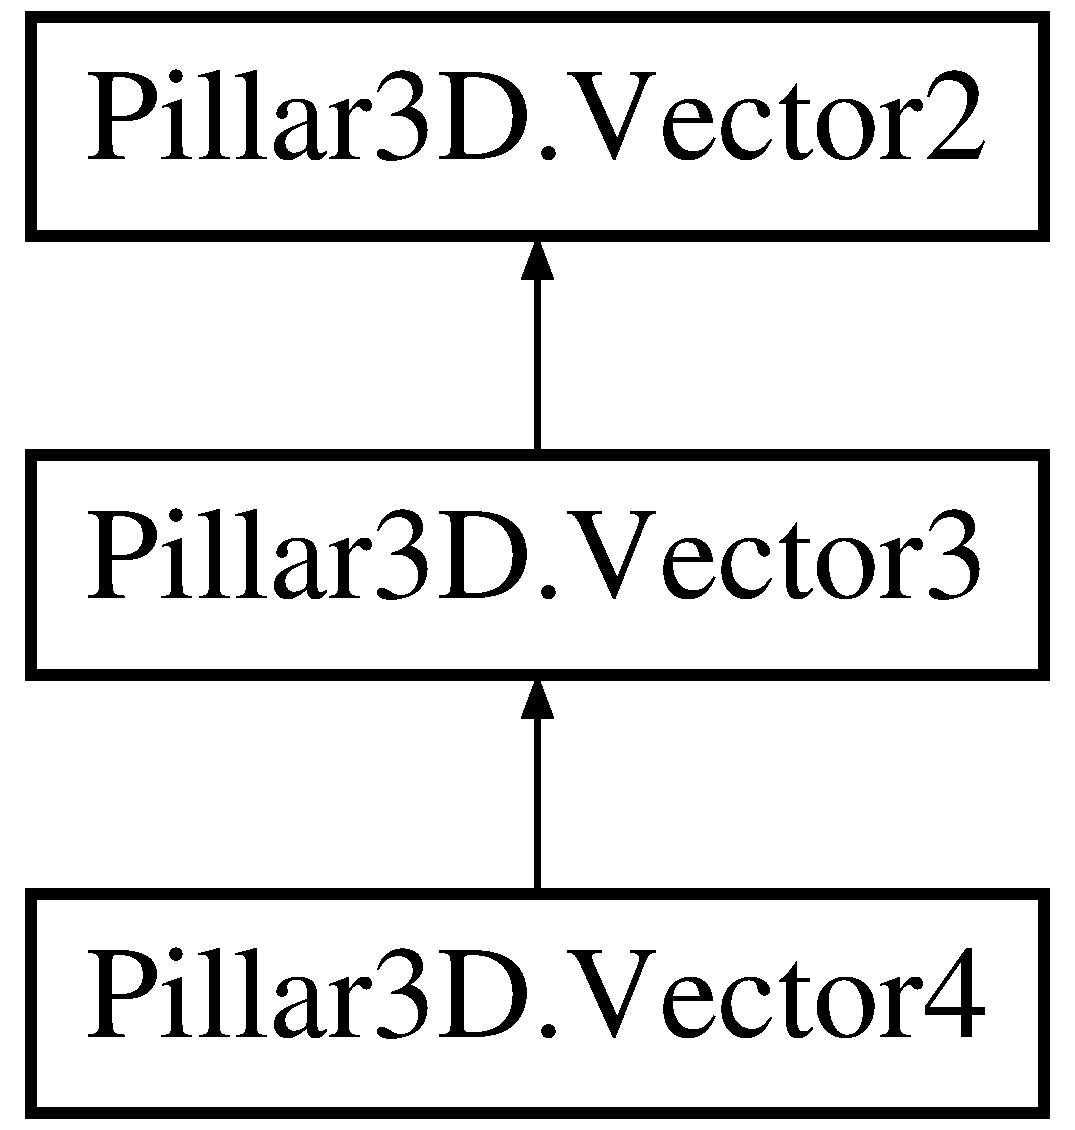
\includegraphics[height=3.000000cm]{class_pillar3_d_1_1_vector3}
\end{center}
\end{figure}
\subsection*{Public Member Functions}
\begin{DoxyCompactItemize}
\item 
\mbox{\Hypertarget{class_pillar3_d_1_1_vector3_a44cbb02c26ce15969a2d75a16607618d}\label{class_pillar3_d_1_1_vector3_a44cbb02c26ce15969a2d75a16607618d}} 
{\bfseries Vector3} (float x, float y, float z)
\item 
\mbox{\Hypertarget{class_pillar3_d_1_1_vector3_adfa9028294445953a719ada637eea96f}\label{class_pillar3_d_1_1_vector3_adfa9028294445953a719ada637eea96f}} 
{\bfseries Vector3} (\hyperlink{class_pillar3_d_1_1_vector3}{Vector3} original)
\item 
\mbox{\Hypertarget{class_pillar3_d_1_1_vector3_aab563750d002b183a1eb6327f9807f91}\label{class_pillar3_d_1_1_vector3_aab563750d002b183a1eb6327f9807f91}} 
{\bfseries Vector3} (\hyperlink{class_pillar3_d_1_1_vector2}{Vector2} original)
\item 
\mbox{\Hypertarget{class_pillar3_d_1_1_vector3_aefae9512d036dd1a7765fa3fb1d56581}\label{class_pillar3_d_1_1_vector3_aefae9512d036dd1a7765fa3fb1d56581}} 
new float {\bfseries Magnitude} ()
\item 
\mbox{\Hypertarget{class_pillar3_d_1_1_vector3_a0cb349a385d9e4cc42df2056f64824e5}\label{class_pillar3_d_1_1_vector3_a0cb349a385d9e4cc42df2056f64824e5}} 
new float {\bfseries Sqr\+Magnitude} ()
\item 
\mbox{\Hypertarget{class_pillar3_d_1_1_vector3_adfbc811e52af952f655a7794e8f06325}\label{class_pillar3_d_1_1_vector3_adfbc811e52af952f655a7794e8f06325}} 
new \hyperlink{class_pillar3_d_1_1_vector3}{Vector3} {\bfseries Normalize} ()
\item 
\mbox{\Hypertarget{class_pillar3_d_1_1_vector3_ae85877f86f52a771377ad5b0635b762f}\label{class_pillar3_d_1_1_vector3_ae85877f86f52a771377ad5b0635b762f}} 
new \hyperlink{class_pillar3_d_1_1_vector3}{Vector3} {\bfseries Normalized} ()
\item 
\mbox{\Hypertarget{class_pillar3_d_1_1_vector3_a99b6ac01b7b55fb6e50148f3a7fde0b7}\label{class_pillar3_d_1_1_vector3_a99b6ac01b7b55fb6e50148f3a7fde0b7}} 
override string {\bfseries To\+String} ()
\end{DoxyCompactItemize}
\subsection*{Static Public Member Functions}
\begin{DoxyCompactItemize}
\item 
\mbox{\Hypertarget{class_pillar3_d_1_1_vector3_a342f16886fd42f3badbe65f74e4aff71}\label{class_pillar3_d_1_1_vector3_a342f16886fd42f3badbe65f74e4aff71}} 
static float {\bfseries Dot} (\hyperlink{class_pillar3_d_1_1_vector3}{Vector3} lhs, \hyperlink{class_pillar3_d_1_1_vector3}{Vector3} rhs)
\item 
\mbox{\Hypertarget{class_pillar3_d_1_1_vector3_a52a5fe672b103b07c734ab6942545415}\label{class_pillar3_d_1_1_vector3_a52a5fe672b103b07c734ab6942545415}} 
static float {\bfseries Angle} (\hyperlink{class_pillar3_d_1_1_vector3}{Vector3} lhs, \hyperlink{class_pillar3_d_1_1_vector3}{Vector3} rhs)
\item 
\mbox{\Hypertarget{class_pillar3_d_1_1_vector3_a64eb77c8785e1c17a53b8e8d4b4b7b64}\label{class_pillar3_d_1_1_vector3_a64eb77c8785e1c17a53b8e8d4b4b7b64}} 
static \hyperlink{class_pillar3_d_1_1_vector3}{Vector3} {\bfseries Cross} (\hyperlink{class_pillar3_d_1_1_vector3}{Vector3} lhs, \hyperlink{class_pillar3_d_1_1_vector3}{Vector3} rhs)
\item 
\mbox{\Hypertarget{class_pillar3_d_1_1_vector3_ab234d7716c916baa088d1c150c4e58c7}\label{class_pillar3_d_1_1_vector3_ab234d7716c916baa088d1c150c4e58c7}} 
static \hyperlink{class_pillar3_d_1_1_vector3}{Vector3} {\bfseries Lerp} (\hyperlink{class_pillar3_d_1_1_vector3}{Vector3} a, \hyperlink{class_pillar3_d_1_1_vector3}{Vector3} b, float t)
\item 
\mbox{\Hypertarget{class_pillar3_d_1_1_vector3_a2ccf06ff68c6532cd81a336bc647079c}\label{class_pillar3_d_1_1_vector3_a2ccf06ff68c6532cd81a336bc647079c}} 
static \hyperlink{class_pillar3_d_1_1_vector3}{Vector3} {\bfseries operator$\ast$} (\hyperlink{class_pillar3_d_1_1_vector3}{Vector3} lhs, float rhs)
\item 
\mbox{\Hypertarget{class_pillar3_d_1_1_vector3_a8c6fbd22e06cb2bd3fd9fd73c63a758a}\label{class_pillar3_d_1_1_vector3_a8c6fbd22e06cb2bd3fd9fd73c63a758a}} 
static \hyperlink{class_pillar3_d_1_1_vector3}{Vector3} {\bfseries operator$\ast$} (float lhs, \hyperlink{class_pillar3_d_1_1_vector3}{Vector3} rhs)
\item 
\mbox{\Hypertarget{class_pillar3_d_1_1_vector3_a6c10b598f20a4db4c12a26d102480472}\label{class_pillar3_d_1_1_vector3_a6c10b598f20a4db4c12a26d102480472}} 
static \hyperlink{class_pillar3_d_1_1_vector3}{Vector3} {\bfseries operator/} (\hyperlink{class_pillar3_d_1_1_vector3}{Vector3} lhs, float rhs)
\item 
\mbox{\Hypertarget{class_pillar3_d_1_1_vector3_ab572845b7172a6dd0aae1d032eaaa742}\label{class_pillar3_d_1_1_vector3_ab572845b7172a6dd0aae1d032eaaa742}} 
static \hyperlink{class_pillar3_d_1_1_vector3}{Vector3} {\bfseries operator+} (\hyperlink{class_pillar3_d_1_1_vector3}{Vector3} lhs, \hyperlink{class_pillar3_d_1_1_vector3}{Vector3} rhs)
\item 
\mbox{\Hypertarget{class_pillar3_d_1_1_vector3_a4d60f3b74aeb32a8de93a2200898dafa}\label{class_pillar3_d_1_1_vector3_a4d60f3b74aeb32a8de93a2200898dafa}} 
static \hyperlink{class_pillar3_d_1_1_vector3}{Vector3} {\bfseries operator-\/} (\hyperlink{class_pillar3_d_1_1_vector3}{Vector3} lhs, \hyperlink{class_pillar3_d_1_1_vector3}{Vector3} rhs)
\item 
\mbox{\Hypertarget{class_pillar3_d_1_1_vector3_afefce7156e7a7d139422b8b3e0018871}\label{class_pillar3_d_1_1_vector3_afefce7156e7a7d139422b8b3e0018871}} 
static \hyperlink{class_pillar3_d_1_1_vector3}{Vector3} {\bfseries operator$\ast$} (\hyperlink{class_pillar3_d_1_1_quaternion}{Quaternion} q, \hyperlink{class_pillar3_d_1_1_vector3}{Vector3} v)
\item 
\mbox{\Hypertarget{class_pillar3_d_1_1_vector3_a6f7f86abdae888eaecd405b3e9535a7a}\label{class_pillar3_d_1_1_vector3_a6f7f86abdae888eaecd405b3e9535a7a}} 
static \hyperlink{class_pillar3_d_1_1_vector3}{Vector3} {\bfseries operator$\ast$} (\hyperlink{class_pillar3_d_1_1_vector3}{Vector3} lhs, \hyperlink{class_pillar3_d_1_1_vector3}{Vector3} rhs)
\item 
\mbox{\Hypertarget{class_pillar3_d_1_1_vector3_aba9e4899693fe5bdbc27daed1fe644cb}\label{class_pillar3_d_1_1_vector3_aba9e4899693fe5bdbc27daed1fe644cb}} 
static \hyperlink{class_pillar3_d_1_1_vector3}{Vector3} {\bfseries operator/} (\hyperlink{class_pillar3_d_1_1_vector3}{Vector3} lhs, \hyperlink{class_pillar3_d_1_1_vector3}{Vector3} rhs)
\end{DoxyCompactItemize}
\subsection*{Properties}
\begin{DoxyCompactItemize}
\item 
\mbox{\Hypertarget{class_pillar3_d_1_1_vector3_aceb120fd0db7a008aa271626fc09d9f3}\label{class_pillar3_d_1_1_vector3_aceb120fd0db7a008aa271626fc09d9f3}} 
float {\bfseries z}\hspace{0.3cm}{\ttfamily  \mbox{[}get, set\mbox{]}}
\item 
\mbox{\Hypertarget{class_pillar3_d_1_1_vector3_a21747c815d16081f44fc9a0cce700244}\label{class_pillar3_d_1_1_vector3_a21747c815d16081f44fc9a0cce700244}} 
new float {\bfseries this\mbox{[}int i\mbox{]}}\hspace{0.3cm}{\ttfamily  \mbox{[}get, set\mbox{]}}
\item 
\mbox{\Hypertarget{class_pillar3_d_1_1_vector3_af4ad08d4bee6db34f0bd7b3af7e9379b}\label{class_pillar3_d_1_1_vector3_af4ad08d4bee6db34f0bd7b3af7e9379b}} 
static \hyperlink{class_pillar3_d_1_1_vector3}{Vector3} {\bfseries Forward}\hspace{0.3cm}{\ttfamily  \mbox{[}get\mbox{]}}
\item 
\mbox{\Hypertarget{class_pillar3_d_1_1_vector3_aa88710a6800a719541bfed3a2243b1b7}\label{class_pillar3_d_1_1_vector3_aa88710a6800a719541bfed3a2243b1b7}} 
new static \hyperlink{class_pillar3_d_1_1_vector3}{Vector3} {\bfseries Up} = new \hyperlink{class_pillar3_d_1_1_vector3}{Vector3}(0, 0, 1)\hspace{0.3cm}{\ttfamily  \mbox{[}get\mbox{]}}
\item 
\mbox{\Hypertarget{class_pillar3_d_1_1_vector3_a08e5428b06bb0918c30a04f8efd0a725}\label{class_pillar3_d_1_1_vector3_a08e5428b06bb0918c30a04f8efd0a725}} 
new static \hyperlink{class_pillar3_d_1_1_vector3}{Vector3} {\bfseries Right} = new \hyperlink{class_pillar3_d_1_1_vector3}{Vector3}(0, 1, 0)\hspace{0.3cm}{\ttfamily  \mbox{[}get\mbox{]}}
\item 
\mbox{\Hypertarget{class_pillar3_d_1_1_vector3_aa1bfdf9ab78f6abdfea59e408985cbf8}\label{class_pillar3_d_1_1_vector3_aa1bfdf9ab78f6abdfea59e408985cbf8}} 
static \hyperlink{class_pillar3_d_1_1_vector3}{Vector3} {\bfseries Back} = new \hyperlink{class_pillar3_d_1_1_vector3}{Vector3}(1, 0, 0)\hspace{0.3cm}{\ttfamily  \mbox{[}get\mbox{]}}
\item 
\mbox{\Hypertarget{class_pillar3_d_1_1_vector3_a79b6acc304d0f20f87442b4fa5594ccf}\label{class_pillar3_d_1_1_vector3_a79b6acc304d0f20f87442b4fa5594ccf}} 
new static \hyperlink{class_pillar3_d_1_1_vector3}{Vector3} {\bfseries Down} = new \hyperlink{class_pillar3_d_1_1_vector3}{Vector3}(0, 0, -\/1)\hspace{0.3cm}{\ttfamily  \mbox{[}get\mbox{]}}
\item 
\mbox{\Hypertarget{class_pillar3_d_1_1_vector3_a8cbeef4bf46be68324fc01a54e143373}\label{class_pillar3_d_1_1_vector3_a8cbeef4bf46be68324fc01a54e143373}} 
new static \hyperlink{class_pillar3_d_1_1_vector3}{Vector3} {\bfseries Left} = new \hyperlink{class_pillar3_d_1_1_vector3}{Vector3}(0, -\/1, 0)\hspace{0.3cm}{\ttfamily  \mbox{[}get\mbox{]}}
\item 
\mbox{\Hypertarget{class_pillar3_d_1_1_vector3_a4ec6880b35fb7c5d5b08995ccaa64b6b}\label{class_pillar3_d_1_1_vector3_a4ec6880b35fb7c5d5b08995ccaa64b6b}} 
new static \hyperlink{class_pillar3_d_1_1_vector3}{Vector3} {\bfseries One} = new \hyperlink{class_pillar3_d_1_1_vector3}{Vector3}(-\/1, 0, 0)\hspace{0.3cm}{\ttfamily  \mbox{[}get\mbox{]}}
\item 
\mbox{\Hypertarget{class_pillar3_d_1_1_vector3_ac522dc75adc0b8fd966a305a606a6156}\label{class_pillar3_d_1_1_vector3_ac522dc75adc0b8fd966a305a606a6156}} 
new static \hyperlink{class_pillar3_d_1_1_vector3}{Vector3} {\bfseries Zero} = new \hyperlink{class_pillar3_d_1_1_vector3}{Vector3}(1, 1, 1)\hspace{0.3cm}{\ttfamily  \mbox{[}get\mbox{]}}
\end{DoxyCompactItemize}
\subsection*{Additional Inherited Members}


The documentation for this class was generated from the following file\+:\begin{DoxyCompactItemize}
\item 
C\+:/\+Users/gaben/\+Documents/\+Visual Studio 2015/\+Projects/\+Pillar/\+Pillar/\+Internal/Vector3.\+cs\end{DoxyCompactItemize}

\hypertarget{class_pillar3_d_1_1_vector4}{}\section{Pillar3\+D.\+Vector4 Class Reference}
\label{class_pillar3_d_1_1_vector4}\index{Pillar3\+D.\+Vector4@{Pillar3\+D.\+Vector4}}
Inheritance diagram for Pillar3\+D.\+Vector4\+:\begin{figure}[H]
\begin{center}
\leavevmode
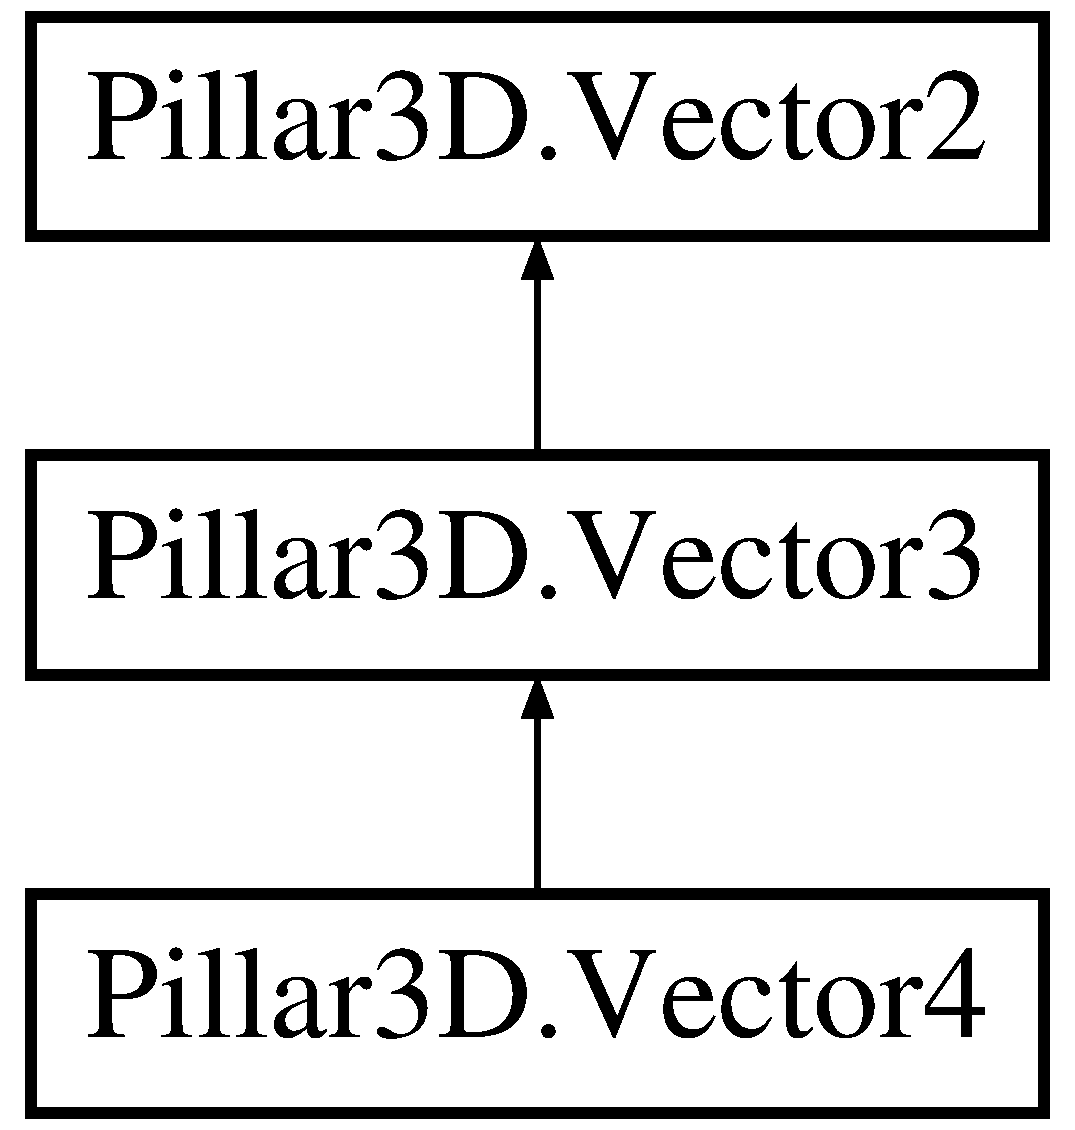
\includegraphics[height=3.000000cm]{class_pillar3_d_1_1_vector4}
\end{center}
\end{figure}
\subsection*{Public Member Functions}
\begin{DoxyCompactItemize}
\item 
\mbox{\Hypertarget{class_pillar3_d_1_1_vector4_afcc54cf1d28b1e7535147dd255224b8e}\label{class_pillar3_d_1_1_vector4_afcc54cf1d28b1e7535147dd255224b8e}} 
{\bfseries Vector4} (float x, float y, float z, float w)
\item 
\mbox{\Hypertarget{class_pillar3_d_1_1_vector4_a7acc452f978c93668f6334c3bda5b68a}\label{class_pillar3_d_1_1_vector4_a7acc452f978c93668f6334c3bda5b68a}} 
{\bfseries Vector4} (\hyperlink{class_pillar3_d_1_1_vector4}{Vector4} original)
\item 
\mbox{\Hypertarget{class_pillar3_d_1_1_vector4_a138582725390583137522f13463cd782}\label{class_pillar3_d_1_1_vector4_a138582725390583137522f13463cd782}} 
{\bfseries Vector4} (\hyperlink{class_pillar3_d_1_1_vector3}{Vector3} original)
\item 
\mbox{\Hypertarget{class_pillar3_d_1_1_vector4_a0c408a4d670de0aaa4f76ecc39ac0412}\label{class_pillar3_d_1_1_vector4_a0c408a4d670de0aaa4f76ecc39ac0412}} 
{\bfseries Vector4} (\hyperlink{class_pillar3_d_1_1_vector2}{Vector2} original)
\item 
\mbox{\Hypertarget{class_pillar3_d_1_1_vector4_a3cbe4c38a1c560c706ae5a4639e7ffd8}\label{class_pillar3_d_1_1_vector4_a3cbe4c38a1c560c706ae5a4639e7ffd8}} 
new float {\bfseries Magnitude} ()
\item 
\mbox{\Hypertarget{class_pillar3_d_1_1_vector4_a964a402e31f2f797b7506c993f0c9c92}\label{class_pillar3_d_1_1_vector4_a964a402e31f2f797b7506c993f0c9c92}} 
new float {\bfseries Sqr\+Magnitude} ()
\item 
\mbox{\Hypertarget{class_pillar3_d_1_1_vector4_a0f22c7eb9ab01e943c47d2f474ad6a09}\label{class_pillar3_d_1_1_vector4_a0f22c7eb9ab01e943c47d2f474ad6a09}} 
new \hyperlink{class_pillar3_d_1_1_vector4}{Vector4} {\bfseries Normalize} ()
\item 
\mbox{\Hypertarget{class_pillar3_d_1_1_vector4_a8bf784854a980006bf21fc40bccacc08}\label{class_pillar3_d_1_1_vector4_a8bf784854a980006bf21fc40bccacc08}} 
new \hyperlink{class_pillar3_d_1_1_vector4}{Vector4} {\bfseries Normalized} ()
\item 
\mbox{\Hypertarget{class_pillar3_d_1_1_vector4_a11b8735a211e3dd543620940e817b9ac}\label{class_pillar3_d_1_1_vector4_a11b8735a211e3dd543620940e817b9ac}} 
override string {\bfseries To\+String} ()
\end{DoxyCompactItemize}
\subsection*{Static Public Member Functions}
\begin{DoxyCompactItemize}
\item 
\mbox{\Hypertarget{class_pillar3_d_1_1_vector4_ad7bf765a6379e75f50997f5243a01307}\label{class_pillar3_d_1_1_vector4_ad7bf765a6379e75f50997f5243a01307}} 
static float {\bfseries Dot} (\hyperlink{class_pillar3_d_1_1_vector4}{Vector4} lhs, \hyperlink{class_pillar3_d_1_1_vector4}{Vector4} rhs)
\item 
\mbox{\Hypertarget{class_pillar3_d_1_1_vector4_a111140c88d27ed39977df085389920d8}\label{class_pillar3_d_1_1_vector4_a111140c88d27ed39977df085389920d8}} 
static float {\bfseries Angle} (\hyperlink{class_pillar3_d_1_1_vector4}{Vector4} lhs, \hyperlink{class_pillar3_d_1_1_vector4}{Vector4} rhs)
\item 
\mbox{\Hypertarget{class_pillar3_d_1_1_vector4_a8c0602c2ddc4119562f6cc5f9161aca1}\label{class_pillar3_d_1_1_vector4_a8c0602c2ddc4119562f6cc5f9161aca1}} 
static \hyperlink{class_pillar3_d_1_1_vector4}{Vector4} {\bfseries Lerp} (\hyperlink{class_pillar3_d_1_1_vector4}{Vector4} a, \hyperlink{class_pillar3_d_1_1_vector4}{Vector4} b, float t)
\item 
\mbox{\Hypertarget{class_pillar3_d_1_1_vector4_ac35cf77fecbf6ccbfbd977c19d08c051}\label{class_pillar3_d_1_1_vector4_ac35cf77fecbf6ccbfbd977c19d08c051}} 
static \hyperlink{class_pillar3_d_1_1_vector4}{Vector4} {\bfseries operator$\ast$} (\hyperlink{class_pillar3_d_1_1_vector4}{Vector4} lhs, float rhs)
\item 
\mbox{\Hypertarget{class_pillar3_d_1_1_vector4_a2f1c74d706834b9212a14797cc782940}\label{class_pillar3_d_1_1_vector4_a2f1c74d706834b9212a14797cc782940}} 
static \hyperlink{class_pillar3_d_1_1_vector4}{Vector4} {\bfseries operator$\ast$} (float lhs, \hyperlink{class_pillar3_d_1_1_vector4}{Vector4} rhs)
\item 
\mbox{\Hypertarget{class_pillar3_d_1_1_vector4_a515cb67123fbeb2198a8ca22006f3ade}\label{class_pillar3_d_1_1_vector4_a515cb67123fbeb2198a8ca22006f3ade}} 
static \hyperlink{class_pillar3_d_1_1_vector4}{Vector4} {\bfseries operator/} (\hyperlink{class_pillar3_d_1_1_vector4}{Vector4} lhs, float rhs)
\item 
\mbox{\Hypertarget{class_pillar3_d_1_1_vector4_adde2ca5deb2e784c68655de5ec7695e4}\label{class_pillar3_d_1_1_vector4_adde2ca5deb2e784c68655de5ec7695e4}} 
static \hyperlink{class_pillar3_d_1_1_vector4}{Vector4} {\bfseries operator+} (\hyperlink{class_pillar3_d_1_1_vector4}{Vector4} lhs, \hyperlink{class_pillar3_d_1_1_vector4}{Vector4} rhs)
\item 
\mbox{\Hypertarget{class_pillar3_d_1_1_vector4_a8c79df7ed45d874bffc588fded8e92ce}\label{class_pillar3_d_1_1_vector4_a8c79df7ed45d874bffc588fded8e92ce}} 
static \hyperlink{class_pillar3_d_1_1_vector4}{Vector4} {\bfseries operator-\/} (\hyperlink{class_pillar3_d_1_1_vector4}{Vector4} lhs, \hyperlink{class_pillar3_d_1_1_vector4}{Vector4} rhs)
\item 
\mbox{\Hypertarget{class_pillar3_d_1_1_vector4_a34c76a6cbe111817e0210b20f89b4d1c}\label{class_pillar3_d_1_1_vector4_a34c76a6cbe111817e0210b20f89b4d1c}} 
static \hyperlink{class_pillar3_d_1_1_vector4}{Vector4} {\bfseries operator$\ast$} (\hyperlink{class_pillar3_d_1_1_vector4}{Vector4} lhs, \hyperlink{class_pillar3_d_1_1_vector4}{Vector4} rhs)
\item 
\mbox{\Hypertarget{class_pillar3_d_1_1_vector4_af92df8988fbb92ca343197ec9df2463e}\label{class_pillar3_d_1_1_vector4_af92df8988fbb92ca343197ec9df2463e}} 
static \hyperlink{class_pillar3_d_1_1_vector4}{Vector4} {\bfseries operator/} (\hyperlink{class_pillar3_d_1_1_vector4}{Vector4} lhs, \hyperlink{class_pillar3_d_1_1_vector4}{Vector4} rhs)
\end{DoxyCompactItemize}
\subsection*{Properties}
\begin{DoxyCompactItemize}
\item 
\mbox{\Hypertarget{class_pillar3_d_1_1_vector4_a2d14ea5dc05dde08aebf14259afeabc2}\label{class_pillar3_d_1_1_vector4_a2d14ea5dc05dde08aebf14259afeabc2}} 
float {\bfseries w}\hspace{0.3cm}{\ttfamily  \mbox{[}get, set\mbox{]}}
\item 
\mbox{\Hypertarget{class_pillar3_d_1_1_vector4_a3f752ca954d46d55d52008a05534d02e}\label{class_pillar3_d_1_1_vector4_a3f752ca954d46d55d52008a05534d02e}} 
new float {\bfseries this\mbox{[}int i\mbox{]}}\hspace{0.3cm}{\ttfamily  \mbox{[}get, set\mbox{]}}
\item 
\mbox{\Hypertarget{class_pillar3_d_1_1_vector4_a8f1a2a0bd0fcd6cc71ef7681e3e7d8a2}\label{class_pillar3_d_1_1_vector4_a8f1a2a0bd0fcd6cc71ef7681e3e7d8a2}} 
new static \hyperlink{class_pillar3_d_1_1_vector4}{Vector4} {\bfseries One}\hspace{0.3cm}{\ttfamily  \mbox{[}get\mbox{]}}
\item 
\mbox{\Hypertarget{class_pillar3_d_1_1_vector4_a8662ba4a2c8630be13485e595e0c779a}\label{class_pillar3_d_1_1_vector4_a8662ba4a2c8630be13485e595e0c779a}} 
new static \hyperlink{class_pillar3_d_1_1_vector4}{Vector4} {\bfseries Zero} = new \hyperlink{class_pillar3_d_1_1_vector4}{Vector4}(1, 1, 1, 1)\hspace{0.3cm}{\ttfamily  \mbox{[}get\mbox{]}}
\end{DoxyCompactItemize}
\subsection*{Additional Inherited Members}


The documentation for this class was generated from the following file\+:\begin{DoxyCompactItemize}
\item 
C\+:/\+Users/gaben/\+Documents/\+Visual Studio 2015/\+Projects/\+Pillar/\+Pillar/\+Internal/Vector3.\+cs\end{DoxyCompactItemize}

\hypertarget{class_pillar3_d_1_1_vector_n}{}\section{Pillar3\+D.\+VectorN Class Reference}
\label{class_pillar3_d_1_1_vector_n}\index{Pillar3\+D.\+VectorN@{Pillar3\+D.\+VectorN}}
\subsection*{Public Member Functions}
\begin{DoxyCompactItemize}
\item 
\mbox{\Hypertarget{class_pillar3_d_1_1_vector_n_a874738a4b57eceb342596dce62b6218c}\label{class_pillar3_d_1_1_vector_n_a874738a4b57eceb342596dce62b6218c}} 
{\bfseries VectorN} (int dimension)
\item 
\mbox{\Hypertarget{class_pillar3_d_1_1_vector_n_a060053d25b1bc1ec00ce8fcc19714f80}\label{class_pillar3_d_1_1_vector_n_a060053d25b1bc1ec00ce8fcc19714f80}} 
{\bfseries VectorN} (params float\mbox{[}$\,$\mbox{]} initial\+Values)
\item 
\mbox{\Hypertarget{class_pillar3_d_1_1_vector_n_ae419187cd84c1500e97e8e45608e3700}\label{class_pillar3_d_1_1_vector_n_ae419187cd84c1500e97e8e45608e3700}} 
override string {\bfseries To\+String} ()
\item 
\mbox{\Hypertarget{class_pillar3_d_1_1_vector_n_a8873ca858d99a7e53dc19a5a59e056d1}\label{class_pillar3_d_1_1_vector_n_a8873ca858d99a7e53dc19a5a59e056d1}} 
\hyperlink{class_pillar3_d_1_1_matrix}{Matrix} {\bfseries To\+Matrix} ()
\item 
\mbox{\Hypertarget{class_pillar3_d_1_1_vector_n_a3d06a84bb56736f21fbc24d22d6ba0e8}\label{class_pillar3_d_1_1_vector_n_a3d06a84bb56736f21fbc24d22d6ba0e8}} 
override bool {\bfseries Equals} (object other)
\item 
\mbox{\Hypertarget{class_pillar3_d_1_1_vector_n_ac1ccc8682c8787c64778575188334026}\label{class_pillar3_d_1_1_vector_n_ac1ccc8682c8787c64778575188334026}} 
override int {\bfseries Get\+Hash\+Code} ()
\end{DoxyCompactItemize}
\subsection*{Static Public Member Functions}
\begin{DoxyCompactItemize}
\item 
\mbox{\Hypertarget{class_pillar3_d_1_1_vector_n_ab69b269151ce7eee42cba4434c208d78}\label{class_pillar3_d_1_1_vector_n_ab69b269151ce7eee42cba4434c208d78}} 
static float {\bfseries Dot} (\hyperlink{class_pillar3_d_1_1_vector_n}{VectorN} lhs, \hyperlink{class_pillar3_d_1_1_vector_n}{VectorN} rhs)
\item 
\mbox{\Hypertarget{class_pillar3_d_1_1_vector_n_a7faf1f76346937ef20450baf245cff21}\label{class_pillar3_d_1_1_vector_n_a7faf1f76346937ef20450baf245cff21}} 
static \hyperlink{class_pillar3_d_1_1_vector_n}{VectorN} {\bfseries operator$\ast$} (\hyperlink{class_pillar3_d_1_1_vector_n}{VectorN} lhs, \hyperlink{class_pillar3_d_1_1_vector_n}{VectorN} rhs)
\item 
\mbox{\Hypertarget{class_pillar3_d_1_1_vector_n_ab8681d6847a08002d4da00d6be7652fd}\label{class_pillar3_d_1_1_vector_n_ab8681d6847a08002d4da00d6be7652fd}} 
static \hyperlink{class_pillar3_d_1_1_vector_n}{VectorN} {\bfseries operator/} (\hyperlink{class_pillar3_d_1_1_vector_n}{VectorN} lhs, \hyperlink{class_pillar3_d_1_1_vector_n}{VectorN} rhs)
\item 
\mbox{\Hypertarget{class_pillar3_d_1_1_vector_n_a4941d28fd6a5ef9eea946cbb07d78587}\label{class_pillar3_d_1_1_vector_n_a4941d28fd6a5ef9eea946cbb07d78587}} 
static \hyperlink{class_pillar3_d_1_1_vector_n}{VectorN} {\bfseries operator$\ast$} (\hyperlink{class_pillar3_d_1_1_vector_n}{VectorN} lhs, float rhs)
\item 
\mbox{\Hypertarget{class_pillar3_d_1_1_vector_n_a0c691e615ea1e5ed60b43101ff2237b7}\label{class_pillar3_d_1_1_vector_n_a0c691e615ea1e5ed60b43101ff2237b7}} 
static \hyperlink{class_pillar3_d_1_1_vector_n}{VectorN} {\bfseries operator$\ast$} (float lhs, \hyperlink{class_pillar3_d_1_1_vector_n}{VectorN} rhs)
\item 
\mbox{\Hypertarget{class_pillar3_d_1_1_vector_n_a3a38fbf078a619760adba05368b2fd4c}\label{class_pillar3_d_1_1_vector_n_a3a38fbf078a619760adba05368b2fd4c}} 
static \hyperlink{class_pillar3_d_1_1_vector_n}{VectorN} {\bfseries operator/} (\hyperlink{class_pillar3_d_1_1_vector_n}{VectorN} lhs, float rhs)
\item 
\mbox{\Hypertarget{class_pillar3_d_1_1_vector_n_a59aa00dbc7d642c2a0402a8acb6a1547}\label{class_pillar3_d_1_1_vector_n_a59aa00dbc7d642c2a0402a8acb6a1547}} 
static \hyperlink{class_pillar3_d_1_1_vector_n}{VectorN} {\bfseries operator/} (float lhs, \hyperlink{class_pillar3_d_1_1_vector_n}{VectorN} rhs)
\item 
\mbox{\Hypertarget{class_pillar3_d_1_1_vector_n_ac153bb2b726415b7d7d4ab8634dea3a8}\label{class_pillar3_d_1_1_vector_n_ac153bb2b726415b7d7d4ab8634dea3a8}} 
static \hyperlink{class_pillar3_d_1_1_vector_n}{VectorN} {\bfseries operator+} (\hyperlink{class_pillar3_d_1_1_vector_n}{VectorN} lhs, \hyperlink{class_pillar3_d_1_1_vector_n}{VectorN} rhs)
\item 
\mbox{\Hypertarget{class_pillar3_d_1_1_vector_n_a57f2f0bcc2ede6da09a9e4b2d3400cec}\label{class_pillar3_d_1_1_vector_n_a57f2f0bcc2ede6da09a9e4b2d3400cec}} 
static \hyperlink{class_pillar3_d_1_1_vector_n}{VectorN} {\bfseries operator-\/} (\hyperlink{class_pillar3_d_1_1_vector_n}{VectorN} lhs, \hyperlink{class_pillar3_d_1_1_vector_n}{VectorN} rhs)
\item 
\mbox{\Hypertarget{class_pillar3_d_1_1_vector_n_ae9191d514dc4a39e2697b0e35b94d51f}\label{class_pillar3_d_1_1_vector_n_ae9191d514dc4a39e2697b0e35b94d51f}} 
static bool {\bfseries operator==} (\hyperlink{class_pillar3_d_1_1_vector_n}{VectorN} lhs, \hyperlink{class_pillar3_d_1_1_vector_n}{VectorN} rhs)
\item 
\mbox{\Hypertarget{class_pillar3_d_1_1_vector_n_af09186943caceb54b82d63315953acd9}\label{class_pillar3_d_1_1_vector_n_af09186943caceb54b82d63315953acd9}} 
static bool {\bfseries operator!=} (\hyperlink{class_pillar3_d_1_1_vector_n}{VectorN} lhs, \hyperlink{class_pillar3_d_1_1_vector_n}{VectorN} rhs)
\end{DoxyCompactItemize}
\subsection*{Properties}
\begin{DoxyCompactItemize}
\item 
\mbox{\Hypertarget{class_pillar3_d_1_1_vector_n_af24ba0ae6d51fbc85300fcabb4a51102}\label{class_pillar3_d_1_1_vector_n_af24ba0ae6d51fbc85300fcabb4a51102}} 
int {\bfseries Dimension}\hspace{0.3cm}{\ttfamily  \mbox{[}get\mbox{]}}
\item 
\mbox{\Hypertarget{class_pillar3_d_1_1_vector_n_abef4e0c42410558c1f427e53dd1d5c28}\label{class_pillar3_d_1_1_vector_n_abef4e0c42410558c1f427e53dd1d5c28}} 
float {\bfseries this\mbox{[}int i\mbox{]}}\hspace{0.3cm}{\ttfamily  \mbox{[}get, set\mbox{]}}
\end{DoxyCompactItemize}


The documentation for this class was generated from the following file\+:\begin{DoxyCompactItemize}
\item 
C\+:/\+Users/gaben/\+Documents/\+Visual Studio 2015/\+Projects/\+Pillar/\+Pillar/\+Internal/Vector3.\+cs\end{DoxyCompactItemize}

\hypertarget{class_pillar3_d_1_1_rendering_1_1_vulkan_wrapper}{}\section{Pillar3\+D.\+Rendering.\+Vulkan\+Wrapper Class Reference}
\label{class_pillar3_d_1_1_rendering_1_1_vulkan_wrapper}\index{Pillar3\+D.\+Rendering.\+Vulkan\+Wrapper@{Pillar3\+D.\+Rendering.\+Vulkan\+Wrapper}}


The documentation for this class was generated from the following file\+:\begin{DoxyCompactItemize}
\item 
C\+:/\+Users/gaben/\+Documents/\+Visual Studio 2015/\+Projects/\+Pillar/\+Pillar/\+Internal/Vulkan\+Wrapper.\+cs\end{DoxyCompactItemize}

\hypertarget{class_pillar3_d_1_1_coroutines_1_1_wait_for_seconds}{}\section{Pillar3\+D.\+Coroutines.\+Wait\+For\+Seconds Class Reference}
\label{class_pillar3_d_1_1_coroutines_1_1_wait_for_seconds}\index{Pillar3\+D.\+Coroutines.\+Wait\+For\+Seconds@{Pillar3\+D.\+Coroutines.\+Wait\+For\+Seconds}}
Inheritance diagram for Pillar3\+D.\+Coroutines.\+Wait\+For\+Seconds\+:\begin{figure}[H]
\begin{center}
\leavevmode
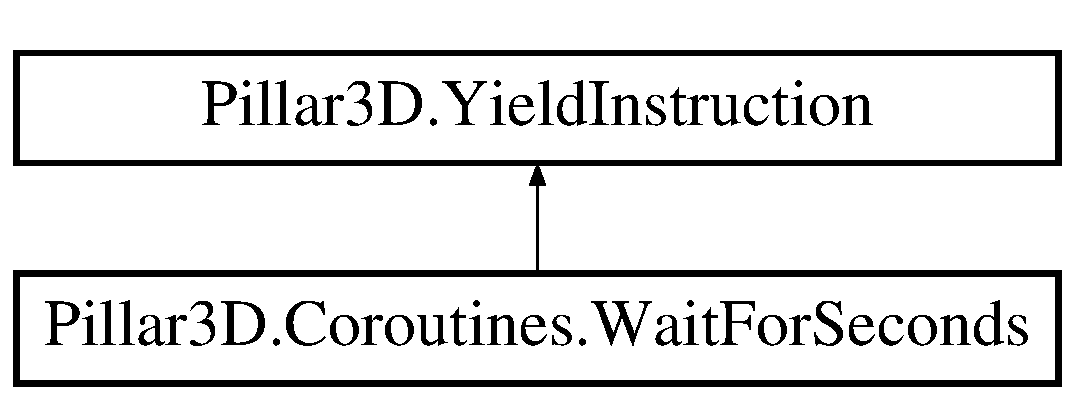
\includegraphics[height=2.000000cm]{class_pillar3_d_1_1_coroutines_1_1_wait_for_seconds}
\end{center}
\end{figure}
\subsection*{Public Member Functions}
\begin{DoxyCompactItemize}
\item 
\mbox{\Hypertarget{class_pillar3_d_1_1_coroutines_1_1_wait_for_seconds_afba40c0c85d2e8ca1810bdee7222a61e}\label{class_pillar3_d_1_1_coroutines_1_1_wait_for_seconds_afba40c0c85d2e8ca1810bdee7222a61e}} 
override Instruction {\bfseries Get\+Instruction} ()
\item 
\mbox{\Hypertarget{class_pillar3_d_1_1_coroutines_1_1_wait_for_seconds_aca45ff32389c27ffed6a998952fab58d}\label{class_pillar3_d_1_1_coroutines_1_1_wait_for_seconds_aca45ff32389c27ffed6a998952fab58d}} 
{\bfseries Wait\+For\+Seconds} (float seconds)
\end{DoxyCompactItemize}


The documentation for this class was generated from the following file\+:\begin{DoxyCompactItemize}
\item 
C\+:/\+Users/gaben/\+Documents/\+Visual Studio 2015/\+Projects/\+Pillar/\+Pillar/\+Internal/Wait\+For\+Seconds.\+cs\end{DoxyCompactItemize}

\hypertarget{class_pillar3_d_1_1_coroutines_1_1_wait_for_seconds_accurate}{}\section{Pillar3\+D.\+Coroutines.\+Wait\+For\+Seconds\+Accurate Class Reference}
\label{class_pillar3_d_1_1_coroutines_1_1_wait_for_seconds_accurate}\index{Pillar3\+D.\+Coroutines.\+Wait\+For\+Seconds\+Accurate@{Pillar3\+D.\+Coroutines.\+Wait\+For\+Seconds\+Accurate}}
Inheritance diagram for Pillar3\+D.\+Coroutines.\+Wait\+For\+Seconds\+Accurate\+:\begin{figure}[H]
\begin{center}
\leavevmode
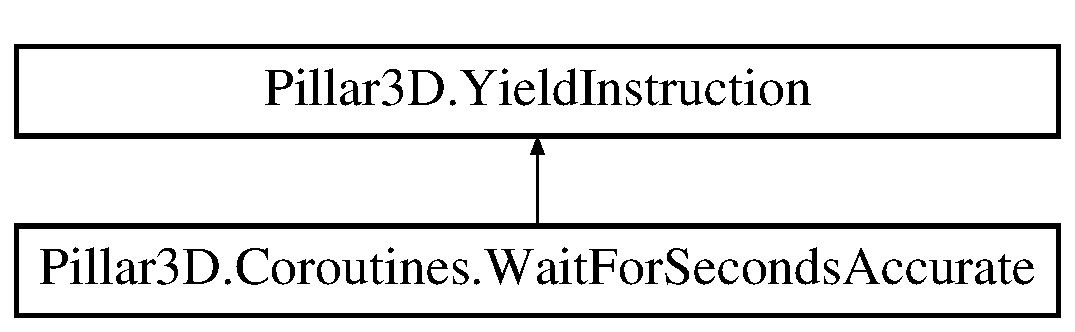
\includegraphics[height=2.000000cm]{class_pillar3_d_1_1_coroutines_1_1_wait_for_seconds_accurate}
\end{center}
\end{figure}
\subsection*{Public Member Functions}
\begin{DoxyCompactItemize}
\item 
\mbox{\Hypertarget{class_pillar3_d_1_1_coroutines_1_1_wait_for_seconds_accurate_a9167921ec6a1a719e5a437c64681bb0d}\label{class_pillar3_d_1_1_coroutines_1_1_wait_for_seconds_accurate_a9167921ec6a1a719e5a437c64681bb0d}} 
override Instruction {\bfseries Get\+Instruction} ()
\item 
\mbox{\Hypertarget{class_pillar3_d_1_1_coroutines_1_1_wait_for_seconds_accurate_a2cbefdf8b00e056b0822874d20fdccf0}\label{class_pillar3_d_1_1_coroutines_1_1_wait_for_seconds_accurate_a2cbefdf8b00e056b0822874d20fdccf0}} 
{\bfseries Wait\+For\+Seconds\+Accurate} (float t)
\end{DoxyCompactItemize}


The documentation for this class was generated from the following file\+:\begin{DoxyCompactItemize}
\item 
C\+:/\+Users/gaben/\+Documents/\+Visual Studio 2015/\+Projects/\+Pillar/\+Pillar/\+Internal/Wait\+For\+Seconds.\+cs\end{DoxyCompactItemize}

\hypertarget{class_pillar3_d_1_1_coroutines_1_1_wait_for_seconds_functional}{}\section{Pillar3\+D.\+Coroutines.\+Wait\+For\+Seconds\+Functional Class Reference}
\label{class_pillar3_d_1_1_coroutines_1_1_wait_for_seconds_functional}\index{Pillar3\+D.\+Coroutines.\+Wait\+For\+Seconds\+Functional@{Pillar3\+D.\+Coroutines.\+Wait\+For\+Seconds\+Functional}}
Inheritance diagram for Pillar3\+D.\+Coroutines.\+Wait\+For\+Seconds\+Functional\+:\begin{figure}[H]
\begin{center}
\leavevmode
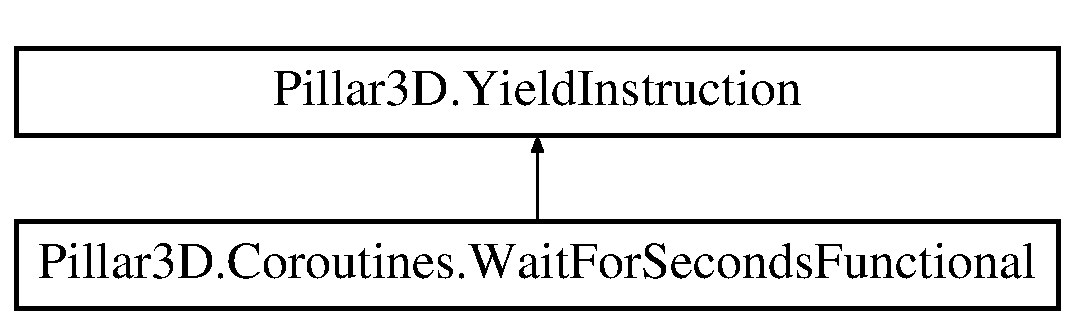
\includegraphics[height=2.000000cm]{class_pillar3_d_1_1_coroutines_1_1_wait_for_seconds_functional}
\end{center}
\end{figure}
\subsection*{Public Member Functions}
\begin{DoxyCompactItemize}
\item 
\mbox{\Hypertarget{class_pillar3_d_1_1_coroutines_1_1_wait_for_seconds_functional_a52fca86896bf2218d50f27b24ee2119c}\label{class_pillar3_d_1_1_coroutines_1_1_wait_for_seconds_functional_a52fca86896bf2218d50f27b24ee2119c}} 
{\bfseries Wait\+For\+Seconds\+Functional} (float time, Action$<$ float $>$ actor)
\item 
\mbox{\Hypertarget{class_pillar3_d_1_1_coroutines_1_1_wait_for_seconds_functional_aa14879cb65f6b98935b8cc7cd7bc7405}\label{class_pillar3_d_1_1_coroutines_1_1_wait_for_seconds_functional_aa14879cb65f6b98935b8cc7cd7bc7405}} 
override Instruction {\bfseries Get\+Instruction} ()
\end{DoxyCompactItemize}


The documentation for this class was generated from the following file\+:\begin{DoxyCompactItemize}
\item 
C\+:/\+Users/gaben/\+Documents/\+Visual Studio 2015/\+Projects/\+Pillar/\+Pillar/\+Internal/Wait\+For\+Seconds.\+cs\end{DoxyCompactItemize}

\hypertarget{class_pillar3_d_1_1_coroutines_1_1_wait_for_seconds_interruptable}{}\section{Pillar3\+D.\+Coroutines.\+Wait\+For\+Seconds\+Interruptable Class Reference}
\label{class_pillar3_d_1_1_coroutines_1_1_wait_for_seconds_interruptable}\index{Pillar3\+D.\+Coroutines.\+Wait\+For\+Seconds\+Interruptable@{Pillar3\+D.\+Coroutines.\+Wait\+For\+Seconds\+Interruptable}}
Inheritance diagram for Pillar3\+D.\+Coroutines.\+Wait\+For\+Seconds\+Interruptable\+:\begin{figure}[H]
\begin{center}
\leavevmode
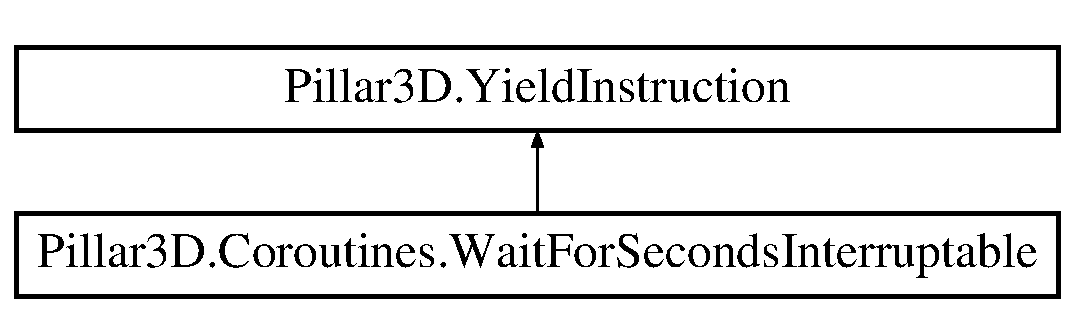
\includegraphics[height=2.000000cm]{class_pillar3_d_1_1_coroutines_1_1_wait_for_seconds_interruptable}
\end{center}
\end{figure}
\subsection*{Public Member Functions}
\begin{DoxyCompactItemize}
\item 
\mbox{\Hypertarget{class_pillar3_d_1_1_coroutines_1_1_wait_for_seconds_interruptable_acfdee8aeadb5a28acf02e8abcff4e69f}\label{class_pillar3_d_1_1_coroutines_1_1_wait_for_seconds_interruptable_acfdee8aeadb5a28acf02e8abcff4e69f}} 
override Instruction {\bfseries Get\+Instruction} ()
\item 
\mbox{\Hypertarget{class_pillar3_d_1_1_coroutines_1_1_wait_for_seconds_interruptable_a3583ccebaafeb2f92d270310cf6aa0eb}\label{class_pillar3_d_1_1_coroutines_1_1_wait_for_seconds_interruptable_a3583ccebaafeb2f92d270310cf6aa0eb}} 
{\bfseries Wait\+For\+Seconds\+Interruptable} (float time, Func$<$ bool $>$ predicate)
\end{DoxyCompactItemize}


The documentation for this class was generated from the following file\+:\begin{DoxyCompactItemize}
\item 
C\+:/\+Users/gaben/\+Documents/\+Visual Studio 2015/\+Projects/\+Pillar/\+Pillar/\+Internal/Wait\+For\+Seconds.\+cs\end{DoxyCompactItemize}

\hypertarget{class_pillar3_d_1_1_coroutines_1_1_wait_for_seconds_unscaled}{}\section{Pillar3\+D.\+Coroutines.\+Wait\+For\+Seconds\+Unscaled Class Reference}
\label{class_pillar3_d_1_1_coroutines_1_1_wait_for_seconds_unscaled}\index{Pillar3\+D.\+Coroutines.\+Wait\+For\+Seconds\+Unscaled@{Pillar3\+D.\+Coroutines.\+Wait\+For\+Seconds\+Unscaled}}
Inheritance diagram for Pillar3\+D.\+Coroutines.\+Wait\+For\+Seconds\+Unscaled\+:\begin{figure}[H]
\begin{center}
\leavevmode
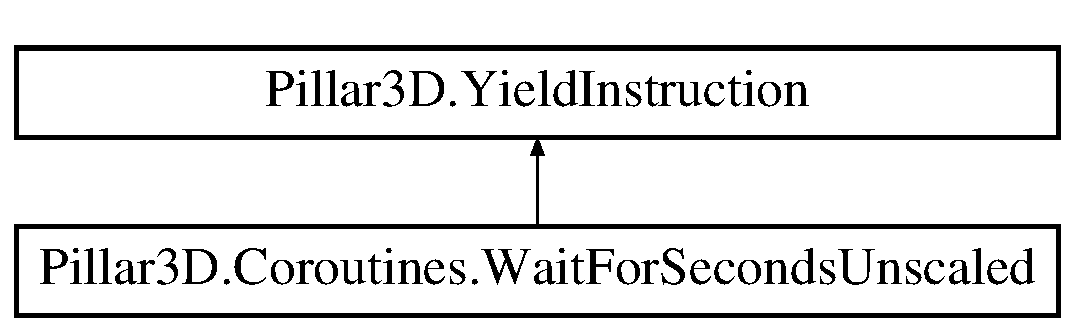
\includegraphics[height=2.000000cm]{class_pillar3_d_1_1_coroutines_1_1_wait_for_seconds_unscaled}
\end{center}
\end{figure}
\subsection*{Public Member Functions}
\begin{DoxyCompactItemize}
\item 
\mbox{\Hypertarget{class_pillar3_d_1_1_coroutines_1_1_wait_for_seconds_unscaled_aa119ae1160297b5d8541f95c9831315f}\label{class_pillar3_d_1_1_coroutines_1_1_wait_for_seconds_unscaled_aa119ae1160297b5d8541f95c9831315f}} 
override Instruction {\bfseries Get\+Instruction} ()
\item 
\mbox{\Hypertarget{class_pillar3_d_1_1_coroutines_1_1_wait_for_seconds_unscaled_af52b3d2728cdf7f1039c1e101dbf0c9d}\label{class_pillar3_d_1_1_coroutines_1_1_wait_for_seconds_unscaled_af52b3d2728cdf7f1039c1e101dbf0c9d}} 
{\bfseries Wait\+For\+Seconds\+Unscaled} (float seconds)
\end{DoxyCompactItemize}


The documentation for this class was generated from the following file\+:\begin{DoxyCompactItemize}
\item 
C\+:/\+Users/gaben/\+Documents/\+Visual Studio 2015/\+Projects/\+Pillar/\+Pillar/\+Internal/Wait\+For\+Seconds.\+cs\end{DoxyCompactItemize}

\hypertarget{class_pillar3_d_1_1_coroutines_1_1_wait_until}{}\section{Pillar3\+D.\+Coroutines.\+Wait\+Until Class Reference}
\label{class_pillar3_d_1_1_coroutines_1_1_wait_until}\index{Pillar3\+D.\+Coroutines.\+Wait\+Until@{Pillar3\+D.\+Coroutines.\+Wait\+Until}}
Inheritance diagram for Pillar3\+D.\+Coroutines.\+Wait\+Until\+:\begin{figure}[H]
\begin{center}
\leavevmode
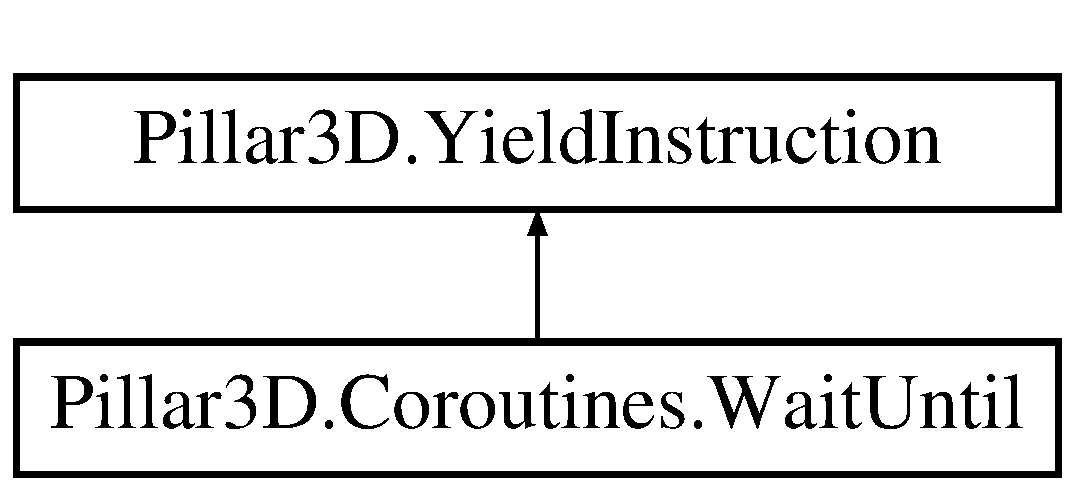
\includegraphics[height=2.000000cm]{class_pillar3_d_1_1_coroutines_1_1_wait_until}
\end{center}
\end{figure}
\subsection*{Public Member Functions}
\begin{DoxyCompactItemize}
\item 
\mbox{\Hypertarget{class_pillar3_d_1_1_coroutines_1_1_wait_until_a400f383b129ff0ec9845936c74a3d4b1}\label{class_pillar3_d_1_1_coroutines_1_1_wait_until_a400f383b129ff0ec9845936c74a3d4b1}} 
override Instruction {\bfseries Get\+Instruction} ()
\item 
\mbox{\Hypertarget{class_pillar3_d_1_1_coroutines_1_1_wait_until_a12236029f97f334f0aa7d670ece9d3b1}\label{class_pillar3_d_1_1_coroutines_1_1_wait_until_a12236029f97f334f0aa7d670ece9d3b1}} 
{\bfseries Wait\+Until} (Func$<$ bool $>$ condition)
\end{DoxyCompactItemize}


The documentation for this class was generated from the following file\+:\begin{DoxyCompactItemize}
\item 
C\+:/\+Users/gaben/\+Documents/\+Visual Studio 2015/\+Projects/\+Pillar/\+Pillar/\+Internal/Wait\+For\+Seconds.\+cs\end{DoxyCompactItemize}

\hypertarget{class_pillar3_d_1_1_coroutines_1_1_wait_while}{}\section{Pillar3\+D.\+Coroutines.\+Wait\+While Class Reference}
\label{class_pillar3_d_1_1_coroutines_1_1_wait_while}\index{Pillar3\+D.\+Coroutines.\+Wait\+While@{Pillar3\+D.\+Coroutines.\+Wait\+While}}
Inheritance diagram for Pillar3\+D.\+Coroutines.\+Wait\+While\+:\begin{figure}[H]
\begin{center}
\leavevmode
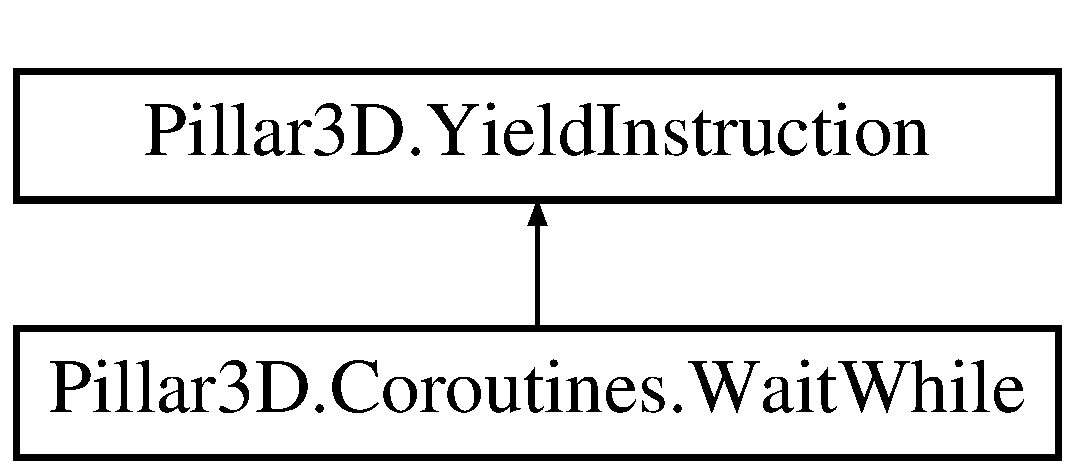
\includegraphics[height=2.000000cm]{class_pillar3_d_1_1_coroutines_1_1_wait_while}
\end{center}
\end{figure}
\subsection*{Public Member Functions}
\begin{DoxyCompactItemize}
\item 
\mbox{\Hypertarget{class_pillar3_d_1_1_coroutines_1_1_wait_while_a6c9bb5a9f850d252bc0b023f5f5e73cf}\label{class_pillar3_d_1_1_coroutines_1_1_wait_while_a6c9bb5a9f850d252bc0b023f5f5e73cf}} 
override Instruction {\bfseries Get\+Instruction} ()
\item 
\mbox{\Hypertarget{class_pillar3_d_1_1_coroutines_1_1_wait_while_a15f4bc0de915f36a57f6dff0f64e0d49}\label{class_pillar3_d_1_1_coroutines_1_1_wait_while_a15f4bc0de915f36a57f6dff0f64e0d49}} 
{\bfseries Wait\+While} (Func$<$ bool $>$ condition)
\end{DoxyCompactItemize}


The documentation for this class was generated from the following file\+:\begin{DoxyCompactItemize}
\item 
C\+:/\+Users/gaben/\+Documents/\+Visual Studio 2015/\+Projects/\+Pillar/\+Pillar/\+Internal/Wait\+For\+Seconds.\+cs\end{DoxyCompactItemize}

\hypertarget{class_pillar3_d_1_1_yield_instruction}{}\section{Pillar3\+D.\+Yield\+Instruction Class Reference}
\label{class_pillar3_d_1_1_yield_instruction}\index{Pillar3\+D.\+Yield\+Instruction@{Pillar3\+D.\+Yield\+Instruction}}
Inheritance diagram for Pillar3\+D.\+Yield\+Instruction\+:\begin{figure}[H]
\begin{center}
\leavevmode
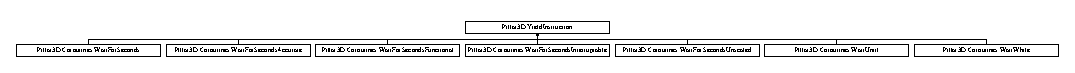
\includegraphics[height=0.536913cm]{class_pillar3_d_1_1_yield_instruction}
\end{center}
\end{figure}
\subsection*{Public Member Functions}
\begin{DoxyCompactItemize}
\item 
\mbox{\Hypertarget{class_pillar3_d_1_1_yield_instruction_a26be5cef50ef706eaa195af4aa36973e}\label{class_pillar3_d_1_1_yield_instruction_a26be5cef50ef706eaa195af4aa36973e}} 
abstract Instruction {\bfseries Get\+Instruction} ()
\end{DoxyCompactItemize}


The documentation for this class was generated from the following file\+:\begin{DoxyCompactItemize}
\item 
C\+:/\+Users/gaben/\+Documents/\+Visual Studio 2015/\+Projects/\+Pillar/\+Pillar/\+Internal/Yield\+Instruction.\+cs\end{DoxyCompactItemize}

%--- End generated contents ---

% Index
\backmatter
\newpage
\phantomsection
\clearemptydoublepage
\addcontentsline{toc}{chapter}{Index}
\printindex

\end{document}
